\documentclass[11pt,openany]{book}
\usepackage[a4paper,margin=2.5cm]{geometry}
\usepackage[T1]{fontenc}
\usepackage{lmodern}
\usepackage{amsmath,amssymb}
\usepackage{booktabs}
\usepackage{array}
\usepackage{microtype}
\emergencystretch=2em
\usepackage{xcolor}
\usepackage{enumitem}
\usepackage{tikz}
\usetikzlibrary{positioning,arrows.meta,shapes.geometric,calc,fit,backgrounds}
\usepackage{pgfplots}
\pgfplotsset{compat=1.18}
\usepackage[most]{tcolorbox}
\usepackage[colorlinks=true,linkcolor=blue!50!black,urlcolor=blue!50!black,citecolor=blue!50!black]{hyperref}

% ---------- colours ----------
\definecolor{ours}{RGB}{31,119,180}
\definecolor{base}{RGB}{170,170,170}
\definecolor{good}{RGB}{44,160,44}
\definecolor{bad}{RGB}{214,39,40}
\definecolor{pend}{RGB}{255,127,14}
\definecolor{soft}{RGB}{240,245,252}

% ---------- boxes ----------
\newtcolorbox{keyidea}[1][]{enhanced,breakable,colback=blue!4,colframe=ours,fonttitle=\bfseries,title={Key idea\ifx\relax#1\relax\else: #1\fi}}
\newtcolorbox{summarybox}{enhanced,breakable,colback=green!4,colframe=good!70!black,fonttitle=\bfseries,title={Chapter summary}}
\newtcolorbox{pendingbox}[1][]{enhanced,breakable,colback=orange!6,colframe=pend,fonttitle=\bfseries,title={In progress -- results pending\ifx\relax#1\relax\else: #1\fi}}
\newtcolorbox{warnbox}[1][]{enhanced,breakable,colback=red!4,colframe=bad!80!black,fonttitle=\bfseries,title={#1}}
\newtcolorbox{bestbox}{enhanced,breakable,colback=yellow!8,colframe=black!60,fonttitle=\bfseries,title={The current best method, in one paragraph}}

% ---------- helpers ----------
\newcommand{\sig}{\ensuremath{^\dagger}}
\newcommand{\code}[1]{\texttt{#1}}
\newcommand{\qsec}{\section*{The question}}
\newcommand{\tsec}{\section*{What we tried}}
\newcommand{\wsec}{\section*{Why}}
\newcommand{\hsec}{\section*{What happened}}
\newcommand{\lsec}{\section*{What we learned}}
\setlist{itemsep=2pt,topsep=4pt}
\renewcommand{\arraystretch}{1.15}

\title{\Huge Teaching a Video Model to See the Right Pairs\\[0.6em]
\Large A textbook account of one research project:\\ beating a video scene-graph model on three benchmarks, honestly}
\author{Project notes, written up for curious readers}
\date{October 2026}

\begin{document}
\frontmatter
\maketitle

\chapter*{How to read this book}
This book tells the full story of a research project, from the first question to the experiments that are still running as these
pages are written. It is meant for a bright high-school student who knows some algebra and has heard of ``AI'', but has never
trained a neural network. Every idea is explained from scratch the first time it appears, and there is a glossary at the end.

The project had a simple goal: take a published video model called \textbf{TraSeR}, which describes videos as \emph{scene
graphs}, and build something that does better on three standard tests (``benchmarks''). The interesting part is not only
\emph{what} we built, but \emph{how we kept ourselves honest} while building it. Science is full of results that look good only
because the researcher, without meaning to, tuned the method to the test. A large part of this book is about the rules we set
ourselves to avoid that trap, and about the many ideas that \emph{failed} those rules. Failures are reported as carefully as
successes, because they are where most of the learning happened.

Most of the story chapters in Part~II follow the same pattern:
\begin{itemize}
  \item \textbf{The question} -- what we wanted to know;
  \item \textbf{What we tried} -- the experiment;
  \item \textbf{Why} -- the reasoning that made it worth trying;
  \item \textbf{What happened} -- the numbers;
  \item \textbf{What we learned} -- what the numbers mean for the next step.
\end{itemize}
Blue boxes contain key ideas, green boxes summarise a chapter, and orange boxes mark experiments whose results were not yet in
when this book was written.

\paragraph{A note on numbers.} Every number in this book comes from the project's research log. All comparisons with TraSeR
are made against \emph{our own reproduction} of TraSeR, scored with \emph{our own} evaluation code and our own automatic judge
(Chapter~\ref{ch:measure}). The TraSeR paper used a different judge, so its printed numbers are not directly comparable with ours;
we only ever compare systems scored in the same way. Small differences of $\pm 0.1$ between tables (for example a baseline F1 of
21.3 in one place and 21.4 in another) come from the judge's memory of past decisions being merged between runs; they do not
change any conclusion.

\tableofcontents

\mainmatter
% =====================================================================
\part{Foundations}
% =====================================================================

\chapter{The problem and the answer, in brief}\label{ch:intro}

Look at a short video of a person riding a horse. You do not just see ``a person'' and ``a horse''. You see that the person is
\emph{on} the horse, is \emph{holding} the reins, is \emph{wearing} a hat, and that all of this is true from second 0 to second 8.
A \textbf{video scene graph} writes exactly this kind of understanding down in a form a computer can check.

\begin{figure}[h]
\centering
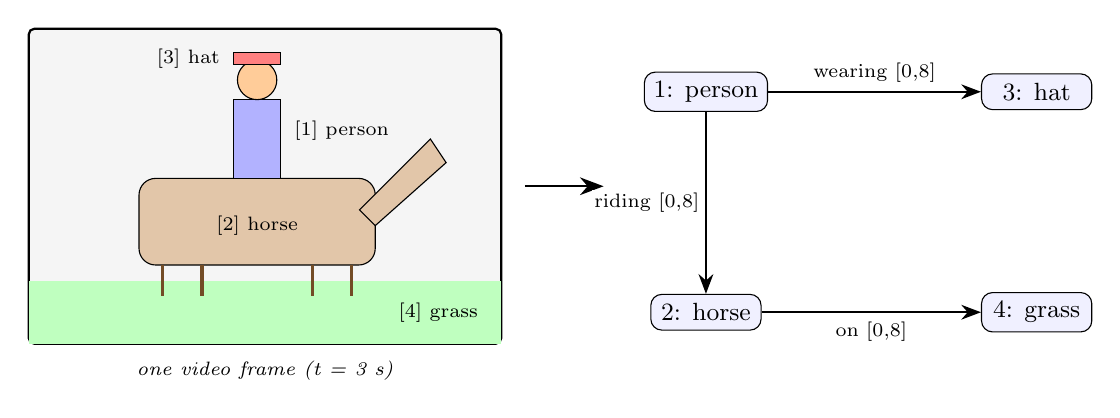
\begin{tikzpicture}[font=\small]
  % frame
  \draw[thick,rounded corners=2pt,fill=gray!8] (0,0) rectangle (6,4);
  \node[anchor=north,font=\scriptsize\itshape] at (3,-0.1) {one video frame (t = 3 s)};
  % ground
  \fill[green!25] (0,0) rectangle (6,0.8);
  \node[font=\scriptsize] at (5.2,0.4) {[4] grass};
  % horse
  \draw[fill=brown!45,rounded corners=6pt] (1.4,1.0) rectangle (4.4,2.1);
  \draw[fill=brown!45] (4.2,1.7) -- (5.1,2.6) -- (5.3,2.3) -- (4.4,1.5) -- cycle;
  \foreach \x in {1.7,2.2,3.6,4.1} \draw[very thick,brown!60!black] (\x,1.0) -- (\x,0.6);
  \node[font=\scriptsize] at (2.9,1.5) {[2] horse};
  % person
  \draw[fill=blue!30] (2.6,2.1) rectangle (3.2,3.1);
  \draw[fill=orange!40] (2.9,3.35) circle (0.25);
  \node[font=\scriptsize,anchor=west] at (3.25,2.7) {[1] person};
  % hat
  \draw[fill=red!50] (2.6,3.55) rectangle (3.2,3.7);
  \node[font=\scriptsize,anchor=east] at (2.55,3.62) {[3] hat};
  % arrow
  \draw[-{Stealth[length=3mm]},thick] (6.3,2) -- (7.3,2);
  % graph
  \begin{scope}[xshift=7.8cm,yshift=0cm,every node/.style={draw,rounded corners,fill=blue!6,minimum width=1.4cm,font=\small}]
    \node (p) at (0.8,3.2) {1: person};
    \node (h) at (0.8,0.4) {2: horse};
    \node (hat) at (5.0,3.2) {3: hat};
    \node (g) at (5.0,0.4) {4: grass};
  \end{scope}
  \begin{scope}[-{Stealth[length=2.5mm]},thick,every node/.style={font=\scriptsize,fill=white,inner sep=1pt}]
    \draw (p) -- node[left=1pt] {riding [0,8]} (h);
    \draw (p) -- node[above=2pt] {wearing [0,8]} (hat);
    \draw (h) -- node[below=2pt] {on [0,8]} (g);
  \end{scope}
\end{tikzpicture}
\caption{A toy video frame and the scene graph that describes it. Each object has an id and a name. Each relation is an
arrow from a \emph{subject} to an \emph{object}, labelled with a \emph{predicate} (``riding'') and the time span in seconds during
which it holds (``[0,8]'').}
\label{fig:toygraph}
\end{figure}

Formally, a video scene graph is:
\begin{itemize}
  \item a list of \textbf{objects}, each with an id and a name (``1: person'', ``2: horse''), and sometimes attributes
  (``brown'', ``standing'');
  \item a list of \textbf{relations}, each written as a quadruple
  \[ [\,\text{subject id},\ \text{predicate},\ \text{object id},\ \text{time spans}\,], \]
  for example \code{[1, "riding", 2, [[0, 8]]]}. A relation may hold during several separate spans, such as
  \code{[[0,3],[6,9]]}.
\end{itemize}
A combination \emph{(subject name, predicate, object name)} such as \emph{(person, riding, horse)} is called a \textbf{triplet}.

\section*{The setting of this project}
In the version of the task studied here, the computer is \emph{given} the objects: every object comes with a ``mask'', a pixel
outline of where it is in every frame. The model's job is to (1) name each object and (2) write down the relations between them,
with time spans. The answer is written as a piece of structured text in the JSON format, which looks like this:
\begin{verbatim}
{"objects": [{"object 1": "person"}, {"object 2": "horse"}, ...],
 "relationships": [[1, "riding", 2, [[0, 8]]],
                   [1, "wearing", 3, [[0, 8]]], ...]}
\end{verbatim}

\textbf{TraSeR} is a recently published model for exactly this task. Our goal was to beat it on three benchmarks --
\textbf{SVG2test}, \textbf{VidOR} and \textbf{PVSG} -- while obeying strict rules of fairness (Chapter~\ref{ch:rules}). The most
important rule: we may only train on \emph{the same training data TraSeR was trained on}, and we must use \emph{one} model with
\emph{one} configuration for all three benchmarks.

\begin{bestbox}
Our best system has two parts that work together. First, TraSeR is improved with \textbf{whole-graph reinforcement learning}
(called \textbf{G3}): it writes many candidate scene graphs for training videos, each is scored against the training labels, and
the model is nudged towards the better ones. Second, a small \textbf{geometry ranker} looks at the object masks and proposes pairs
of objects that probably have a relation but that the graph never mentioned; a separately trained \textbf{pair decoder}
(called \textbf{PG}, trained by reinforcement learning on single pairs, and allowed to answer ``no relation'') describes each
proposed pair. The two outputs are merged. Compared with TraSeR, this system finds significantly more of the true relations on all
three benchmarks (relation recall 24.7$\to$36.9 on SVG2test, 9.2$\to$12.1 on VidOR, 9.7$\to$14.1 on PVSG), finds significantly
more fully correct triplets on all three, and has a higher F1 score on all three, though the F1 gain is statistically clear only
on VidOR. The details are in Chapter~\ref{ch:best}.
\end{bestbox}

\section*{Roadmap}
Part~I (Chapters~\ref{ch:intro}--\ref{ch:rules}) explains the tools: what a vision-language model is, how TraSeR works, how
fine-tuning and reinforcement learning change a model, how results are measured, and which rules we followed. Part~II tells the
story in the order it happened: first we measured where TraSeR fails, then we tried tricks that need no training, then we built a
fast inference engine, then we discovered that the three benchmarks disagree about how relations should be written, then we
trained models, and finally we combined the pieces. Part~III covers what did not work, what is still running, and where the
project could go next.

\begin{summarybox}
A video scene graph lists the objects in a video and the relations between them, with time spans. TraSeR is a published model
for this task. We tried to beat it on three benchmarks using only its own training data and one configuration for everything.
The best system combines whole-graph reinforcement learning (G3) with extra object pairs proposed by a geometry ranker and
described by a pair-level reinforcement-learned decoder (PG).
\end{summarybox}

% ---------------------------------------------------------------------
\chapter{Vision-language models and TraSeR}\label{ch:vlm}

\section{Tokens: how a language model reads and writes}
A \textbf{language model} is a program that, given a piece of text, predicts what comes next. It does not work on letters or
whole words but on \textbf{tokens}: short chunks of text such as ``rid'', ``ing'', ``\{'' or `` horse''. A sentence of ten words
might be fifteen tokens. The model writes text one token at a time: it computes a probability for every possible next token,
picks one, appends it, and repeats. Always picking the most probable token is called \textbf{greedy decoding}; picking at random
according to the probabilities is called \textbf{sampling}. A \textbf{temperature} setting makes sampling more or less adventurous.

Inside, the model is a huge function with billions of adjustable numbers called \textbf{parameters} (or weights). ``Training''
means adjusting these numbers so that the model's predictions get better on examples.

\section{From text to video: vision-language models}
A \textbf{vision-language model} (VLM) is a language model that can also look at images or videos. A separate ``vision encoder''
cuts each frame into small patches and turns each patch into a vector of numbers -- a \emph{visual token}. These visual tokens are
placed in the model's input next to ordinary text tokens, so the language model can ``read'' the picture as if it were text.
TraSeR is built on \textbf{Qwen2.5-VL-3B}, a vision-language model with about 3~billion parameters.

\section{TraSeR's idea: one block of tokens per object}
A video has far too many patches to feed them all to the model. TraSeR's main idea is to \emph{arrange} the visual tokens by
object. Using the given masks, it collects, for each object, the visual information along that object's \emph{trajectory}
(its path through the video) and compresses it into a fixed-size \textbf{object block} of tokens. The input then looks like
Figure~\ref{fig:traser}: an instruction, then the block for object~1, the block for object~2, and so on. The model then writes the
scene graph as text, referring to objects by their position in this list.

\begin{figure}[h]
\centering
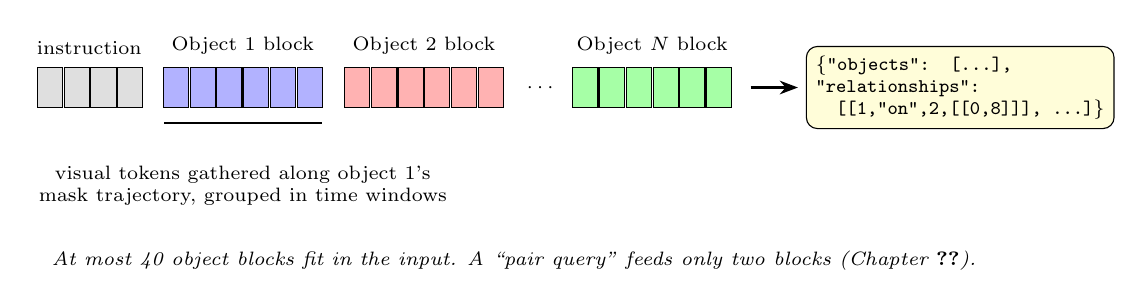
\begin{tikzpicture}[font=\scriptsize,
  tok/.style={draw,minimum width=0.32cm,minimum height=0.5cm,inner sep=0},
  lab/.style={font=\scriptsize}]
  % prompt
  \foreach \i in {0,...,3} \node[tok,fill=gray!25] at (\i*0.34,0) {};
  \node[lab,above] at (0.5,0.3) {instruction};
  % object 1
  \foreach \i in {0,...,5} \node[tok,fill=blue!30] at (1.6+\i*0.34,0) {};
  \node[lab,above] at (2.45,0.3) {Object 1 block};
  % object 2
  \foreach \i in {0,...,5} \node[tok,fill=red!30] at (3.9+\i*0.34,0) {};
  \node[lab,above] at (4.75,0.3) {Object 2 block};
  \node at (6.25,0) {$\cdots$};
  % object N
  \foreach \i in {0,...,5} \node[tok,fill=green!35] at (6.8+\i*0.34,0) {};
  \node[lab,above] at (7.65,0.3) {Object $N$ block};
  % output
  \draw[-{Stealth},thick] (8.9,0) -- (9.5,0);
  \node[draw,rounded corners,fill=yellow!15,align=left,font=\scriptsize\ttfamily,anchor=west] at (9.6,0)
     {\{"objects": [\ldots],\\ "relationships":\\ \ \ [[1,"on",2,[[0,8]]], \ldots]\}};
  % detail of a block
  \draw[decorate,thick] (1.45,-0.45) -- (3.45,-0.45);
  \node[align=center,font=\scriptsize] at (2.45,-1.25)
     {visual tokens gathered along object 1's\\ mask trajectory, grouped in time windows};
  % cap note
  \node[align=left,font=\scriptsize\itshape,anchor=west] at (-0.1,-2.2)
     {At most 40 object blocks fit in the input. A ``pair query'' feeds only two blocks (Chapter~\ref{ch:pairs}).};
\end{tikzpicture}
\caption{TraSeR's input layout: an instruction followed by one block of visual tokens per object. The output is the scene graph,
written as JSON text, which refers to objects by their position in the list of blocks.}
\label{fig:traser}
\end{figure}

Two practical details matter later:
\begin{itemize}
  \item TraSeR accepts at most \textbf{40 objects}. On SVG2test, 7\% of the true relations involve an object beyond this cap.
  \item TraSeR knows two instructions (``prompts''): a \code{scene\_graph} prompt that asks for an open-vocabulary graph in
  SVG2's style, and an older \code{relationships} prompt that was trained on academic datasets with a closed list of predicates.
  We always use the \code{scene\_graph} prompt (Chapter~\ref{ch:salience} shows why).
  \item Because each object is a separate block, we can also feed the model \emph{only two} object blocks and ask ``describe these
  two''. We call this a \textbf{pair query}. It is the backbone of our method.
\end{itemize}

\section{Fine-tuning and LoRA}
TraSeR's weights were already trained. \textbf{Fine-tuning} means continuing training on new examples so the model changes its
behaviour. Changing all 3 billion parameters is expensive and risky. \textbf{LoRA} (Low-Rank Adaptation) is a cheaper trick:
the original weights are frozen, and for some weight matrices $W$ we learn a small correction
\[ W' = W + B A, \]
where $A$ and $B$ are thin matrices. If $W$ is $2048\times 2048$ (about 4 million numbers) and we use ``rank'' $r=64$, then $A$ is
$64\times 2048$ and $B$ is $2048\times 64$, only about 260 thousand numbers. The correction $BA$ is called an \textbf{adapter}.
All our trained models are LoRA adapters of rank 64 on top of the released TraSeR; the released weights are never changed, and
an adapter can be switched on and off.

\section{Two ways to teach: supervised fine-tuning and reinforcement learning}
\paragraph{Supervised fine-tuning (SFT).} We show the model an input and the exact answer we want, and push up the probability of
every token of that answer. This is like a student copying model solutions. It is powerful but literal: the model learns to
imitate the \emph{style} of the answers, including their quirks.

\paragraph{Reinforcement learning (RL).} We let the model write its own answers, give each answer a \textbf{reward} (a score),
and push the model towards answers that scored well. This is like a student who attempts problems and is told only ``that was
better'' or ``that was worse''. It can improve whatever the reward measures, without forcing the model to copy one particular
answer word for word.

\section{GRPO: reinforcement learning by comparing a group of attempts}\label{sec:grpo}
The RL method we use is \textbf{GRPO} (Group Relative Policy Optimisation). For one training input it works like this:
\begin{enumerate}
  \item \textbf{Sample a group.} The model writes $G$ different answers to the same input by sampling (we use $G=8$,
  temperature 1.0).
  \item \textbf{Score each.} A reward function gives each answer a number $r_1,\dots,r_G$.
  \item \textbf{Compute advantages.} Each answer's \textbf{advantage} is its reward minus the group average:
  \[ A_i = r_i - \bar r, \qquad \bar r = \tfrac{1}{G}\textstyle\sum_j r_j. \]
  \item \textbf{Update.} Increase the probability of the tokens of answers with positive advantage, decrease it for negative
  advantage, in proportion to $A_i$.
\end{enumerate}
The group average acts as a fair baseline: an answer is rewarded only for being \emph{better than the model's own typical attempt}
on this input, so easy and hard inputs are treated alike. If all answers in a group get the same reward, every advantage is zero
and nothing is learned from that group.

\begin{keyidea}[A worked GRPO example]
Suppose the model writes 4 scene graphs for one video and the rewards are $0.2,\ 0.5,\ 0.3,\ 0.6$.
The mean is $\bar r = (0.2+0.5+0.3+0.6)/4 = 0.4$. The advantages are
\[ -0.2,\quad +0.1,\quad -0.1,\quad +0.2. \]
So the 4th graph is reinforced most, the 2nd a little, and the 1st and 3rd are discouraged. If instead all four rewards were 0.4,
every advantage would be 0 and the group would teach nothing.
\end{keyidea}

\begin{figure}[h]
\centering
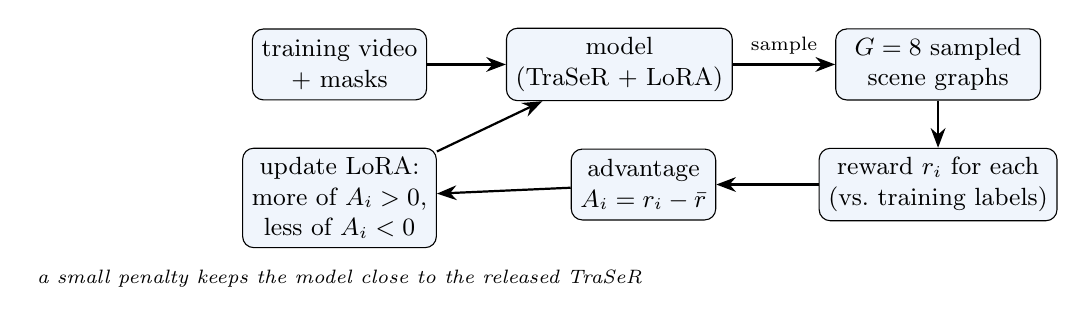
\begin{tikzpicture}[font=\small,node distance=0.6cm and 1.0cm,
  box/.style={draw,rounded corners,fill=soft,minimum height=0.9cm,align=center},
  ar/.style={-{Stealth[length=2.5mm]},thick}]
  \node[box] (in) {training video\\+ masks};
  \node[box,right=of in] (pol) {model\\(TraSeR + LoRA)};
  \node[box,right=1.3cm of pol,minimum width=2.6cm] (s) {$G=8$ sampled\\scene graphs};
  \node[box,below=of s] (r) {reward $r_i$ for each\\(vs.\ training labels)};
  \node[box,left=1.3cm of r] (a) {advantage\\$A_i=r_i-\bar r$};
  \node[box,below=of in] (u) {update LoRA:\\more of $A_i>0$,\\less of $A_i<0$};
  \draw[ar] (in) -- (pol);
  \draw[ar] (pol) -- node[above,font=\scriptsize] {sample} (s);
  \draw[ar] (s) -- (r);
  \draw[ar] (r) -- (a);
  \draw[ar] (a) -- (u);
  \draw[ar] (u) -- (pol);
  \node[font=\scriptsize\itshape,below=0.15cm of u,align=center] {a small penalty keeps the model close to the released TraSeR};
\end{tikzpicture}
\caption{The GRPO loop. Each training step repeats this for a few videos (4 for whole graphs, 16 object pairs for the pair
decoder).}
\label{fig:grpo}
\end{figure}

In our implementation (file \code{engine/grpo.py}) the update is a plain policy-gradient step: the loss is
$-A_i \times(\text{sum of the log-probabilities of answer $i$'s tokens})$, divided by a fixed length, plus (for whole-graph
training) a small penalty with weight $\beta=0.02$ that measures how far the adapted model's token probabilities have drifted from
the released TraSeR. This penalty is a safety rope: it stops the model from wandering into strange behaviour just to please the
reward.

\section{The reward we used}
The reward compares a written scene graph with the training labels of that video (file \code{engine/reward.py}). It is fixed in
advance and is the same for every data source:
\[ R = F1_{\text{rel}} + 0.25 \times \text{object accuracy} - 0.2\times[\text{output is not valid, complete JSON}]. \]
Each predicted relation can be matched to at most one label relation with the same ordered pair of objects and the same
(normalised) predicate; a match earns ``soft'' credit equal to its temporal overlap (defined in the next chapter), a number between
0 and 1. Duplicates cannot match twice, so repeating a relation only lowers precision. $F1_{\text{rel}}$ is computed from these
credits (Chapter~\ref{ch:measure} explains F1).

\begin{summarybox}
Language models read and write tokens. A vision-language model also reads visual tokens. TraSeR arranges visual tokens into one
block per object and writes the scene graph as JSON. We change TraSeR only through small LoRA adapters. Supervised fine-tuning
copies target answers; reinforcement learning rewards good answers. GRPO samples a group of answers, scores them, and pushes the
model towards answers that beat the group's average.
\end{summarybox}

% ---------------------------------------------------------------------
\chapter{How we measure success}\label{ch:measure}

\section{Matching a predicted relation to a true one}
A predicted relation counts as \textbf{correct} (a ``hit'') if there is a true (``ground-truth'', GT) relation such that
\begin{enumerate}
  \item it has the same subject and the same object, in the same order;
  \item its predicate means the same thing -- ``holding'' and ``holds'' should count as equal. An \textbf{LLM judge} (a separate
  language model) decides whether two labels mean the same thing, and its decisions are cached so that the same pair of words is
  always judged the same way;
  \item its time spans overlap the true spans enough: temporal IoU $\ge 0.5$ (below).
\end{enumerate}
Before scoring, exact duplicates of the same (subject, predicate, object) are merged, because a model that repeats itself should
not be scored as if it had said something new. (This turned out to matter: 16\% of TraSeR's relations on SVG2test and 52\% on PVSG
were exact duplicates.)

\section{Precision, recall and F1}
\begin{itemize}
  \item \textbf{Precision} $P$ = (number of correct predictions) / (number of predictions). ``When the model says something, how
  often is it right?''
  \item \textbf{Recall} $R$ = (number of true relations found) / (number of true relations). ``Of everything that is true, how
  much did the model find?''
  \item \textbf{F1} = $\dfrac{2PR}{P+R}$, the harmonic mean. It is high only when \emph{both} are high.
\end{itemize}

\begin{figure}[h]
\centering
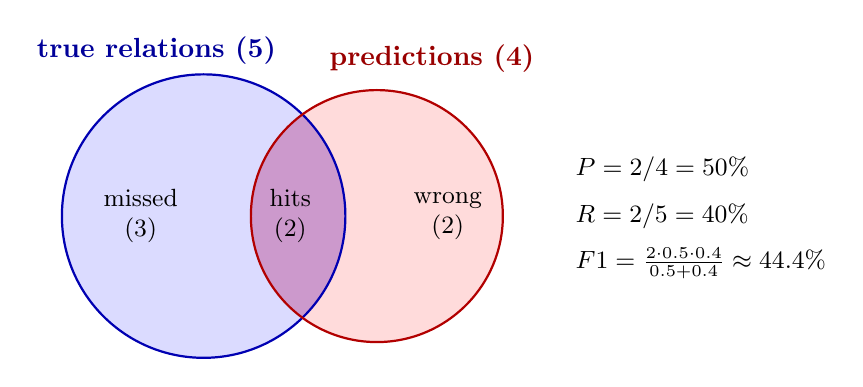
\begin{tikzpicture}[font=\small]
  \fill[blue!20,opacity=0.7] (0,0) circle (1.8);
  \fill[red!20,opacity=0.7] (2.2,0) circle (1.6);
  \begin{scope}
    \clip (0,0) circle (1.8);
    \fill[violet!40] (2.2,0) circle (1.6);
  \end{scope}
  \draw[thick,blue!70!black] (0,0) circle (1.8);
  \draw[thick,red!70!black] (2.2,0) circle (1.6);
  \node[align=center] at (-0.8,0) {missed\\(3)};
  \node[align=center] at (1.1,0) {hits\\(2)};
  \node[align=center] at (3.1,0) {wrong\\(2)};
  \node[blue!60!black,font=\bfseries] at (-0.6,2.1) {true relations (5)};
  \node[red!60!black,font=\bfseries] at (2.9,2.0) {predictions (4)};
  \node[align=left,anchor=west] at (4.6,0.6) {$P = 2/4 = 50\%$};
  \node[align=left,anchor=west] at (4.6,0.0) {$R = 2/5 = 40\%$};
  \node[align=left,anchor=west] at (4.6,-0.6) {$F1 = \frac{2\cdot0.5\cdot0.4}{0.5+0.4}\approx 44.4\%$};
\end{tikzpicture}
\caption{Precision and recall. Precision looks at the red circle (what we said), recall at the blue circle (what is true).}
\label{fig:venn}
\end{figure}

\begin{keyidea}[A worked example]
A video has 5 true relations. The model predicts 4 relations, of which 2 are correct. Then $P=2/4=50\%$, $R=2/5=40\%$ and
$F1 = 2\cdot 0.5\cdot 0.4/(0.5+0.4) = 0.4/0.9 \approx 44.4\%$. If the model adds 4 more guesses and one of them is right, recall
rises to $3/5=60\%$ but precision falls to $3/8=37.5\%$, and F1 becomes $2\cdot0.375\cdot0.6/0.975\approx 46.2\%$ -- a little higher.
Adding guesses helps F1 only if they are right often enough.
\end{keyidea}

A useful rule follows from the formula. Write F1 as $2C/(N_{\text{pred}}+N_{\text{true}})$, where $C$ is the number of hits. Adding
one more prediction that is correct with probability $q$ raises the expected F1 exactly when
\[ \frac{2(C+q)}{N_{\text{pred}}+1+N_{\text{true}}} > \frac{2C}{N_{\text{pred}}+N_{\text{true}}}
   \iff q > \frac{C}{N_{\text{pred}}+N_{\text{true}}} = \frac{F1}{2}. \]
So \emph{an extra relation is worth adding only if its chance of being correct exceeds half the current F1}. We use this rule in
Chapter~\ref{ch:pending}.

\paragraph{Which metric matters?} The official SVG2 metrics are \emph{recall-style}: relation recall, triplet recall and object
accuracy. Recall alone can be gamed by guessing a lot, so we also always report precision and F1.

\section{Temporal IoU: did we get the timing right?}
\textbf{IoU} means ``intersection over union''. For two time intervals, it is the length of the part they share divided by the
length they cover together.

\begin{figure}[h]
\centering
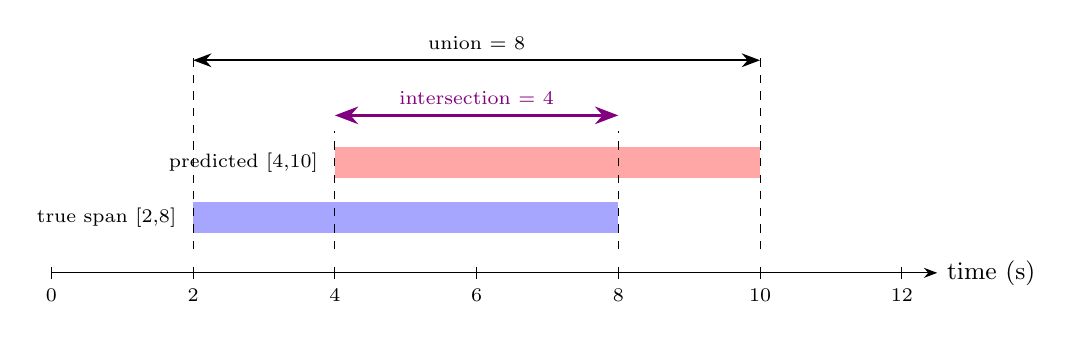
\begin{tikzpicture}[font=\small,x=0.9cm]
  \draw[-{Stealth}] (0,0) -- (12.5,0) node[right] {time (s)};
  \foreach \t in {0,2,...,12} { \draw (\t,0.08) -- (\t,-0.08) node[below,font=\scriptsize] {\t}; }
  \fill[blue!35] (2,0.5) rectangle (8,0.9); \node[anchor=east,font=\scriptsize] at (1.9,0.7) {true span [2,8]};
  \fill[red!35] (4,1.2) rectangle (10,1.6); \node[anchor=east,font=\scriptsize] at (3.9,1.4) {predicted [4,10]};
  \draw[dashed] (4,0.3) -- (4,1.8); \draw[dashed] (8,0.3) -- (8,1.8);
  \draw[violet,very thick,{Stealth}-{Stealth}] (4,2.0) -- node[above,font=\scriptsize] {intersection = 4} (8,2.0);
  \draw[black,thick,{Stealth}-{Stealth}] (2,2.7) -- node[above,font=\scriptsize] {union = 8} (10,2.7);
  \draw[dashed] (2,0.3) -- (2,2.8); \draw[dashed] (10,0.3) -- (10,2.8);
\end{tikzpicture}
\caption{Temporal IoU of the true span [2,8] and the predicted span [4,10]: $4/8=0.5$, exactly at the threshold.}
\label{fig:tiou}
\end{figure}

\begin{keyidea}[Worked tIoU]
True span $[2,8]$, predicted span $[4,10]$. They overlap on $[4,8]$, length 4. Together they cover $[2,10]$, length 8. So
$\text{tIoU}=4/8=0.5$, which just passes the $\ge 0.5$ test. A prediction of $[0,20]$ (``the whole clip'') would overlap all 6
seconds but cover 20, giving $6/20=0.3$: a fail. Lazy ``always true'' spans are punished when the truth is short.
\end{keyidea}

When a relation has several spans, there are two reasonable definitions:
\begin{itemize}
  \item \textbf{per-span}: the relation counts if \emph{some} predicted span matches \emph{some} true span with IoU $\ge 0.5$;
  \item \textbf{union} (merged-span): first merge all spans of each side into one set of seconds, then compute one IoU.
\end{itemize}
These can give very different numbers. On PVSG, TraSeR's relation recall was 6.7 under the union definition, 10.2 per-span, and
24.3 if time is ignored altogether. We use \textbf{per-span tIoU as the primary protocol}, fixed early, and check important claims
under the union definition too.

\section{Triplet recall and object accuracy}
\begin{itemize}
  \item \textbf{Relation recall}: a true relation counts as found if a matching relation is predicted (as above).
  \item \textbf{Triplet recall}: stricter -- the relation must be found \emph{and} both object names must be judged correct.
  A model that finds ``object 1 riding object 2'' but calls the horse a ``cow'' gets relation credit but no triplet credit.
  \item \textbf{Object accuracy}: the share of true objects whose predicted name is judged correct.
\end{itemize}

\section{Confidence intervals by the paired bootstrap}
Suppose system B beats system A by 2 points of recall on 67 videos. Is B really better, or did we get lucky with these 67 videos?
The \textbf{bootstrap} answers this by simulation:
\begin{enumerate}
  \item Compute, for each video, the score of A and of B on that video.
  \item Draw 67 videos \emph{with replacement} from the 67 (some appear twice, some not at all) and compute the difference
  B$-$A on this resampled set.
  \item Repeat 2000 times. Sort the 2000 differences. The middle 95\% (from the 2.5th to the 97.5th percentile) is the
  \textbf{95\% confidence interval} (CI).
\end{enumerate}
It is \textbf{paired} because A and B are always compared on the same resampled videos, which removes the noise of ``this video
is just hard for everyone''. If the whole CI lies above 0, we say the improvement is \emph{significant} and mark it with a dagger,
like this: 36.9\sig. ``n.s.'' means not significant.

\begin{keyidea}[Toy bootstrap]
Three videos give differences B$-$A of $+3, +1, -1$; the mean is $+1$. Resamples might be $\{+3,+3,+1\}$ (mean $+2.3$),
$\{-1,-1,+1\}$ (mean $-0.3$), $\{+1,+3,-1\}$ (mean $+1$), \dots{} With only three videos, many resamples have negative means, so the
interval includes 0: not significant. With 835 videos (VidOR), even small differences become significant if they are
consistent; with 62--67 videos (PVSG, SVG2test) an F1 gain needs to be roughly 3 points to be significant.
\end{keyidea}

The bootstrap only covers \emph{which test videos} we happened to have. It does not cover the randomness of \emph{training}. For
that we retrain with a different random seed (Chapter~\ref{ch:pairs}).

\section{The three benchmarks}
\begin{center}
\small
\begin{tabular}{@{}lccp{5.6cm}@{}}
\toprule
Benchmark & videos & per video & character \\
\midrule
SVG2test (VIPSeg part) & 67 & $\sim$32 relations & human labels, many object \emph{parts} (37--47\% of relations) \\
VidOR (validation) & 835 & 4.8 objects, 36 relations & human labels, closed list of 50 predicates \\
PVSG (validation) & 62 & 20.7 objects, 15.6 relations & human labels, actions, long first-person videos \\
\bottomrule
\end{tabular}
\end{center}
\begin{itemize}
  \item \textbf{SVG2test.} We evaluate the 67-video VIPSeg part. Its labels include parts of objects (``wheel'' of a ``car''),
  and its most common predicates are ``on'', ``wearing'' and ``attached to''.
  \item \textbf{VidOR.} The original labels are boxes, so we converted them to masks with a segmentation model (835 videos, no
  failures). Its annotators state many relations per pair and usually state both directions (Chapter~\ref{ch:conventions}).
  \item \textbf{PVSG.} 62 videos: 40 from VidOR, 11 from Epic-Kitchens, 11 from Ego4D (the last two are first-person videos).
  We discovered that \textbf{35 of the 40 VidOR-sourced PVSG videos are in TraSeR's own training set} -- the baseline has
  already seen them. We therefore also report a \textbf{PVSG-clean} subset of 27 videos that TraSeR never trained on.
\end{itemize}

\begin{summarybox}
A predicted relation is correct if pair, direction, meaning (decided by an LLM judge) and timing (tIoU $\ge 0.5$) all match.
Precision asks how often we are right, recall how much we find, F1 balances both. An extra relation helps F1 only if it is
correct with probability above F1/2. Paired bootstrap intervals tell us whether a difference is real; a dagger \sig{} marks
significance. The three benchmarks have very different labelling styles, and part of PVSG overlaps TraSeR's training data.
\end{summarybox}

% ---------------------------------------------------------------------
\chapter{The rules of the game}\label{ch:rules}

\qsec
How do we make sure that ``we beat TraSeR'' means something? It is surprisingly easy to fool yourself. If you try twenty ideas and
keep the one that scores best \emph{on the test set}, part of its advantage is luck that will not repeat on new data. If you use a
special setting for each benchmark, you are no longer building a general method -- you are fitting the tests.

\section{Rule 1: the same training data as TraSeR}
TraSeR was trained on seven data splits of the SVG2 collection (named PVD, SA-V, VIPSeg, VidOR, VidVRD, LV-VIS and OVIS). We train
\textbf{only} on these. In practice, relation labels exist in PVD (a large split whose labels were written automatically by a large
language model) and the human-labelled VidOR and VidVRD training splits; VIPSeg, LV-VIS and OVIS contain object labels only. Our training runs drew their relation-labelled videos from the PVD and VidOR training splits. Using
extra data (for example PVSG's training set) would make it impossible to tell whether a gain came from our method or from the
data. This rule was set early and confirmed again later: any fix must come from the \emph{method}, not from new data.

\section{Rule 2: one model, one prompt, one configuration}
\begin{keyidea}[Benchmark targeting]
\textbf{Benchmark targeting} means giving the system special knowledge of which test it is taking -- a per-benchmark prompt, a
per-benchmark threshold, a tag like ``this is VidOR, answer VidOR-style'', or a rule copied from one test's labelling habits.
It can raise scores without making the model any better at understanding videos. We forbid it: one model, one prompt, one set of
numbers, applied unchanged to all three benchmarks.
\end{keyidea}
This rule cost us real points. For example, on VidOR, simply adding the reverse direction of every relation raises F1 a lot,
because VidOR's annotators label both directions -- but the same trick hurts SVG2test (Chapter~\ref{ch:conventions}). Under our
rules such a trick is not allowed.

\section{Rule 3: decide on a dev split, with the rule written down first}
We set aside \textbf{40 PVD and 40 VidOR training videos} as a \textbf{dev split} (development set). They are never used for
training. Whenever we must choose between variants, we choose on dev, using a decision rule that is \textbf{written into the log
before the results are seen}. This is called \textbf{pre-registration}.

\begin{keyidea}[Why pre-register?]
Imagine flipping a coin 10 times, seeing 7 heads, and \emph{then} announcing ``my hypothesis was that this coin favours heads''.
That proves nothing. If you announce the hypothesis \emph{first}, then 7 heads is (weak) evidence. Pre-registration forces us to
commit to the test before we know the answer, so we cannot unconsciously move the goalposts. Several of our ideas failed their
pre-registered gate; we report them as failures and did not quietly change the rule.
\end{keyidea}

\section{Rule 4: score test sets once, with uncertainty}
Test sets are used to report results, not to make choices. Each method is scored once, with paired bootstrap confidence intervals
(Chapter~\ref{ch:measure}). When test numbers revealed something during analysis, we only ever used them to \emph{exclude} a method
(the conservative direction), never to add or tune one.

\section{Rule 5: replicate with a second seed}
Training involves randomness: which examples come first, which answers are sampled. A result that appears with seed 0 but not with
seed 1 is fragile. For our main claims we retrained with a second seed.

\section{Rule 6: smoke-test locally before every GPU run}
GPU time is precious: the work ran on a cloud GPU with 96\,GB of memory in sessions of at most 12 hours. Every change was first
tested on a normal computer: on a tiny random copy of the model, or by replaying saved outputs. This caught real bugs. For example,
a proposed rule for stopping runaway output (Chapter~\ref{ch:engine}) was replayed on all 989 saved outputs and turned out to cut
46 perfectly good outputs while missing 10 real loops -- it never reached the GPU.

\section{Rule 7: compare against fair controls}
A gain from ``extra work'' must be compared with the same amount of extra work done in a boring way. We used \emph{random pairs}
as a control for ``smart pairs'', and \emph{plain supervised fine-tuning on the same data} as a control for reinforcement learning.

\section*{Where these rules came from}
The rules were not all there on day one. Early in the project (Chapter~\ref{ch:salience}) we found a training-free trick that
looked great on SVG2test. Then we asked ourselves: ``is this cheating?'' The trick used no test labels, but its two settings had
been picked by looking at SVG2test scores. We wrote down the settings \emph{before} running VidOR -- and on VidOR the trick did
nothing. That failure is the reason the rest of the project is built on pre-registration and dev splits.

\begin{summarybox}
Train only on TraSeR's data. Use one configuration for every benchmark (no benchmark targeting). Choose on a held-out dev split
using rules written down in advance. Score test sets once, with bootstrap intervals. Replicate with a second seed. Smoke-test every
change before using a GPU. Always compare with a fair control.
\end{summarybox}


% =====================================================================
\part{The story}
% =====================================================================

\chapter{The kill test: where does TraSeR fail?}\label{ch:kill}

\qsec
Before inventing a better method, we needed to know \emph{why} TraSeR misses relations. A common guess was ``TraSeR writes too few
relations''. If that were true, the fix would be to make it write more. A \textbf{kill test} is a cheap experiment designed to
kill a hypothesis quickly if it is wrong.

\tsec
We ran the released TraSeR on the 67 VIPSeg videos of SVG2test (one video initially failed on a corrupt frame; this was fixed
later) and, for every true relation it missed, sorted the miss into a category: was the pair of objects never mentioned at all?
Mentioned but with the wrong predicate? Right predicate but wrong time? We also counted how many relations it wrote.

\wsec
Different failure types need different cures. Too few relations needs ``say more''. Wrong pairs needs ``choose better pairs''.
Wrong predicates needs better language. Wrong times needs better timing. Measuring first prevents us from curing the wrong disease.

\hsec
Our reproduction, without a judge, gave a relation recall of 21.7\% (20.5\% strict) -- close to the paper's reported 18.7 on all of
SVG2test, so our evaluation pipeline was calibrated. The breakdown:
\begin{center}
\begin{tabular}{@{}lr@{}}
\toprule
predicted relations per video & \textbf{55.0} (true: 32.1) \\
true relation whose pair was never predicted & 49.8\% (+7.3\% only in the reverse direction) \\
right pair, wrong predicate & 12.9\% \\
right predicate, wrong time & 1.3\% \\
object beyond the 40-object cap & 7.0\% \\
pair-level precision (rough) & 12.7\% \\
\bottomrule
\end{tabular}
\end{center}
TraSeR writes \emph{more} relations than the humans (55 vs 32 per video), so ``too few relations'' was killed immediately. It
heavily over-uses some predicates: ``in front of'' 1527 times (humans: 344), ``cooperating with'' 307 times (humans: about 0).
A look at the data itself showed that humans label only about 2\% of all ordered object pairs (27.8 of roughly 1358 per video),
that 70--75\% of SVG2test relations are static geometry (``on'', ``attached to'') and only 4--8\% are motion, and that using the
whole clip as the time span already gives tIoU $\ge 0.5$ for 72--93\% of the static relations.

\lsec
\begin{keyidea}[The dominant failure is pair selection]
TraSeR talks a lot, but about the \emph{wrong pairs}. Half of the human relations are on pairs it never mentions. Timing is
rarely the problem on SVG2test. So the central question of the project became: \emph{which pairs of objects should the model
talk about?}
\end{keyidea}

\begin{summarybox}
TraSeR writes 55 relations per video where humans write 32, but half the human relations are on object pairs TraSeR never
mentions. The bottleneck is choosing the right pairs, not the number of relations or their timing.
\end{summarybox}

% ---------------------------------------------------------------------
\chapter[Training-free tricks and a reality check]{Training-free tricks: salience, pair queries, and a reality check}\label{ch:salience}

\qsec
If the problem is choosing pairs, can we fix it \emph{without any training}, just by deciding which pairs to ask TraSeR about?
And is such a fix general, or does it only work on the benchmark where we designed it?

\section{Touching pairs are salient}
\tsec
We tested a simple \textbf{salience} prior: pairs whose masks \emph{touch} (after slightly enlarging the masks, in any frame sampled
once per second) are the pairs humans care about.

\wsec
People describe what interacts: the cup \emph{on} the table, the person \emph{holding} the phone. Objects far apart rarely get a
relation. This costs nothing to compute from the masks.

\hsec
At an equal number of pairs per video, choosing touching pairs covered 49.6\% of the human-labelled pairs, versus 43.1\% for
TraSeR's own choice and 13.9\% for random pairs. Humans state a relation for 22.3\% of touching pairs but only 1.4\% of
non-touching pairs; TraSeR states non-touching pairs at 5.9\%, four times the human rate. Dropping all TraSeR relations between
non-touching objects (a \textbf{contact filter}) raised the rough precision from 12.7\% to 20.9\% and F1 from 16.0 to 19.6, while
recall fell from 21.7 to 18.5: 48.6\% of TraSeR's outputs were non-touching pairs, but they contained only 15\% of its hits.

\section{Pair queries: asking about two objects at a time}
\tsec
For the top touching pairs that TraSeR did not mention, we fed TraSeR \emph{only those two object blocks} and asked it to describe
them (a \textbf{pair query}, Figure~\ref{fig:traser}). Its answers were added to the original graph.

\hsec
With an \emph{oracle} predicate (cheating, to measure headroom), adding 10 such pairs per video would raise recall from 21.7 to
29.3, and 20 pairs to 35.3; with 10 pairs, a hand-written rule for the predicate reached only 22.8. With TraSeR's own answers using the older \code{relationships}
prompt, recall rose only to 24.3: the pairs were now covered, but the predicates were wrong. The cause was the prompt: the
\code{relationships} prompt had been trained on academic data with a closed vocabulary, so TraSeR answered ``next to'' 683 times,
and rarely ``on'' -- the most common human predicate on these pairs (143 of about 330). Switching to the open-vocabulary
\code{scene\_graph} prompt fixed this:

\begin{center}
\begin{tabular}{@{}lccc@{}}
\toprule
SVG2test (judge, tIoU $\ge$ .5) & recall & strict recall & relations/video \\
\midrule
TraSeR & 25.1 & 20.5 & 55 \\
+ all objects (no 40 cap) & 25.8 & 21.6 & 65 \\
+ 10 salient pairs (\code{scene\_graph}) & 32.0 & 25.8 & 86 \\
+ 20 salient pairs (\code{scene\_graph}) & 36.2 & 28.8 & 106 \\
+ 20 salient pairs (\code{relationships}) & 33.6 & 23.6 & 109 \\
\bottomrule
\end{tabular}
\end{center}
On the decoded salient pairs, TraSeR got 69\% of the human relations right (272 of 395). Its misses were mostly phrasing in the
other direction (``person in front of clothes'' vs.\ the true ``clothes behind person'') and part--whole relations (``car has
wheel'' vs.\ the true ``wheel near car'').

\section{The control: is it salience or just more decoding?}
\wsec
Asking about 20 extra pairs is extra work. Maybe \emph{any} 20 extra pairs would help as much. The fair control is 20
\emph{random} extra pairs.

\hsec
With the same budget, 20 salient pairs gave recall 30.2 (on a judge-free metric) versus 24.5 for 20 random pairs, starting from
about 22. About 75\% of the gain came from salience, not from extra decoding.

\section{Corrected numbers}
Later we found that TraSeR often repeats exact duplicates (16\% of its relations on SVG2test, 52\% on PVSG), which distorted the
precision numbers. After merging duplicates and using per-span tIoU, the SVG2test table became:
\begin{center}
\begin{tabular}{@{}lccc@{}}
\toprule
SVG2test (deduplicated, per-span) & P & R & F1 \\
\midrule
TraSeR & 16.9 & 24.7 & 20.1 \\
contact filter & 27.4 & 21.9 & 24.3 \\
+ 20 random pairs & 10.4 & 28.0 & 15.1 \\
filter + 20 salient & 16.9 & 32.2 & 22.2 \\
filter + 30 salient & 15.6 & 37.6 & 22.0 \\
+ 40 salient & 12.3 & 43.4 & 19.2 \\
\bottomrule
\end{tabular}
\end{center}
On SVG2test, ``filter + 20 salient'' kept precision equal and raised recall by 7.5 points. On PVSG, however, the same tricks traded
precision for recall rather than improving both (TraSeR P/R/F1 5.8/10.2/7.4; filter + 10 salient 5.1/13.7/7.5; +40 salient
2.9/16.9/5.0), so an earlier claim that the method improved PVSG on every axis was withdrawn.

\section{The reality check on VidOR}\label{sec:vidor-prereg}
\qsec
Was this a general method, or had we tuned it to SVG2test?

\tsec
The number of pairs (20) and the use of the filter had been chosen by looking at SVG2test. So, \emph{before} running VidOR, we
wrote into the log: ``Configuration chosen on SVG2test only: contact filter + top-20 salient touching pairs, \code{scene\_graph}
prompt, duplicates merged. Control: +20 random pairs.'' VidOR would be a held-out test of a fixed configuration.

\hsec
\begin{center}
\begin{tabular}{@{}lcccc@{}}
\toprule
VidOR (835 videos) & P & R & F1 & triplet R \\
\midrule
TraSeR & 27.2 & 9.3 & 13.9 & 6.6 \\
contact filter & 30.6 & 7.2 & 11.7 & 5.2 \\
+ 20 random & 20.0 & 12.0 & 15.0 & 8.2 \\
\textbf{filter + 20 salient (pre-registered)} & 27.2 & 9.1 & 13.6 & 6.3 \\
+ 20 salient & 25.3 & 11.2 & 15.5 & 7.7 \\
\bottomrule
\end{tabular}
\end{center}
The pre-registered configuration did \emph{nothing} on VidOR (recall change $-0.2$, CI $[-0.6, 0.2]$). On VidOR, salient pairs did
not even beat random pairs. VidOR videos have few objects (about 4.8), and VidOR annotators label non-touching relations heavily.
TraSeR's VidOR problems were different: it wrote too \emph{few} relations (12.4 per video vs.\ 36.1 true), 27.8\% of misses were
relations stated only in the other direction, and predicted spans were far too long (median 20\,s vs.\ 4.3\,s true).

\section{Other attempts in this phase}
\begin{itemize}
  \item \textbf{Inverse-direction normalisation} (treat ``A above B'' as also ``B below A''): recall rose by only 0.7--1.4 points
  and precision collapsed (for example P 12.9$\to$8.1). A recall-only trick; not a method.
  \item \textbf{Re-ranking by containment} (prefer pairs where one object sits inside the other -- parts): on SVG2test it helped
  (F1 22.2$\to$23.6), but it had been designed from test analysis, and on PVSG it did not transfer. Salience is protocol-dependent:
  SVG2test labels parts, PVSG does not.
  \item \textbf{Shrinking spans with contact}: cutting TraSeR's spans to the moments when masks touch \emph{hurt} PVSG (recall
  10.2$\to$8.3). Mask contact does not localise human actions.
  \item \textbf{A learned salience ranker} (a small decision-tree model on mask geometry) beat the plain contact rule when trained on
  enough videos -- an idea we returned to in Chapter~\ref{ch:pairs}.
\end{itemize}

\lsec
\begin{keyidea}[Three benchmarks, three conventions]
Each benchmark encodes a different labelling convention, and TraSeR mismatches each one differently. SVG2test: one relation per
pair, touching and part--whole pairs; TraSeR over-generates filler. PVSG: short action spans; TraSeR's spans are 2.7 times too
long. VidOR: closed vocabulary, both directions, many relations per pair; TraSeR under-generates. \emph{No single inference-time
trick beat TraSeR on all three.}
\end{keyidea}
This was the turning point. A method that wins on one benchmark by matching its habits is not what we wanted. We needed gains that
are \emph{independent} of convention, achieved by training on TraSeR's own data, with choices made on dev data.

\begin{summarybox}
Touching pairs are salient, and asking TraSeR about salient pairs one at a time raised SVG2test recall strongly; a random-pair
control showed the gain was mostly due to salience. But a configuration chosen on SVG2test and pre-registered for VidOR failed
there. The benchmarks follow different conventions, so we moved to training-based methods selected on held-out training videos.
\end{summarybox}

% ---------------------------------------------------------------------
\chapter{Engineering interlude: making TraSeR fast}\label{ch:engine}

\qsec
Reinforcement learning needs the model to write \emph{many} scene graphs: 8 samples per video, for hundreds of steps. At the start,
one scene graph took about 30 seconds. A rough estimate for GRPO with 8 sequential samples was about 4 minutes per video, or about
50 hours for 200 steps of 4 videos -- impossible in 12-hour sessions. Could we make inference much faster without changing what the
model writes?

\section{Batching, and why it was slow at first}
The natural speed-up is \textbf{batching}: let the GPU write many sequences at once. A speed test on one video (27 objects) showed
the potential: one sequence ran at 88.3 tokens/s, while 32 copies in parallel reached 1251 tokens/s (14.2$\times$).

But real batches mix videos of different lengths. Shorter inputs must be \textbf{padded} so all rows line up, and with padding the
first batched engine was barely faster than one-at-a-time. Profiling found the culprit: with a padding mask, the attention code of
the software library we used made 8 copies of the model's ``memory'' (the \textbf{KV cache}, which stores what the model has read
so far) at every step for all 36 layers, because the model shares each memory head among 8 query heads. We rewrote this step so
the memory is read once (an exact rewrite: same mathematics, tested to agree to $4.5\times10^{-7}$). Padded steps went from 87.8\,ms
to 28.2\,ms (3.1$\times$ faster).

\section{Runaway outputs and how to stop them safely}
Sometimes TraSeR gets stuck in a loop, repeating attributes (``white'', ``black'', \ldots) or attaching ``cooperating with'' to every
object, until it hits the 8192-token limit. A first loop-stopping rule (stop if a 24-token chunk repeats 4 times) broke quality:
recall fell from 24.7 to 11.4, because legitimate outputs repeat chunks when a scene has several identical objects (many identical
chairs). A second rule was replayed offline on all 989 saved outputs before any GPU use: it would have wrongly stopped 46 clean
outputs and missed 10 loops, so it was discarded. The final rules (an attribute list longer than 30 items; a 300-character chunk
already seen twice inside the relationships section; and a ``novelty stall'' when the last 40 relations contain fewer than 8 new
ones) left SVG2test and VidOR scores unchanged in replay.

\section{Continuous batching and caching}
Two more ideas finished the job:
\begin{itemize}
  \item \textbf{Continuous batching} (the ``SlotDecoder''): when a sequence finishes, its slot is immediately refilled with a new
  one, so a batch never waits for its slowest member. Tested to be identical, token for token, to the standard generation routine.
  \item \textbf{Caching vision features}: pair queries had been re-running the vision encoder on the whole video for every pair
  (1289 times on SVG2test). Computing it once per video cut the pair stage from 679\,s to 108\,s.
\end{itemize}
The whole SVG2test pipeline went from about 3.9 thousand seconds to about 0.5 thousand (about 7.8$\times$), and the scores were
statistically unchanged (P 18.7, R 24.6, F1 21.3 vs.\ 16.9/24.7/20.1 one-at-a-time; bootstrap not significant). From here on, the
\textbf{baseline} we compare against (called \textbf{A0}) is the released TraSeR run through this fast engine; on all three
benchmarks it matched the original one-at-a-time numbers within noise.

\lsec
Speed work is research work: without it, none of the reinforcement learning in the next chapters would fit into 12-hour sessions.
And every speed change was checked for \emph{quality}, because a faster engine that changes the answers would invalidate every
comparison.

\begin{summarybox}
Batching with a corrected attention step, safe loop stopping (tested offline first), continuous batching and caching made TraSeR
about 8 times faster with unchanged scores. The fast-engine baseline A0 is the TraSeR we compare against from now on.
\end{summarybox}

% ---------------------------------------------------------------------
\chapter{Annotation conventions: the benchmarks disagree}\label{ch:conventions}

\qsec
Chapter~\ref{ch:salience} hinted that the three benchmarks label relations differently. How different, exactly? And which
differences are already present in TraSeR's training data?

\tsec
We measured, on training data and on test data, three simple statistics: relations per video, relations per stated pair, and the
share of stated pairs labelled in \emph{both} directions (A--B and B--A).

\hsec
\begin{center}
\small
\begin{tabular}{@{}lccc@{}}
\toprule
source & rel./video & rel.\ per stated pair & both directions \\
\midrule
VidOR training (human) & 23.6 & 2.89 & 79\% \\
VidOR test (human) & 36.1 & 4.88 & 81\% \\
VidVRD training (human) & 18.0 & 4.61 & 99\% \\
SA-V training (automatic labels) & 18.6 & 1.25 & 7\% \\
SVG2test-VIPSeg (human) & 32.1 & 1.25 & 9\% \\
PVSG validation (human) & 15.6 & 1.31 & 2\% \\
\midrule
TraSeR's output on VidOR test & 12.4 & 1.82 & 12\% \\
\bottomrule
\end{tabular}
\end{center}
VidOR and VidVRD annotators write several relations per pair and nearly always both directions. SVG2test, PVSG and the
automatically labelled SVG2 splits write about one relation per pair and almost never both directions. TraSeR saw the VidOR style in
training, but on VidOR test it writes in the dominant automatic-label style.

A later, sharper measurement on the training labels (Chapter~\ref{ch:failures}) found:
\begin{keyidea}[The direction convention]
When a pair has a relation, the \emph{reverse} pair is also labelled \textbf{91.5\%} of the time in VidOR training data, but only
\textbf{13.1\%} of the time in PVD. VidOR even labels the same predicate in both directions when this is semantically odd: ``in front
of'' in both directions for 41\% of such pairs, ``next to'' for 72\%. So a large part of the ``wrong direction'' misses on VidOR is
not a misunderstanding of the video but a difference in \emph{how labels are written}.
\end{keyidea}

We also broke down TraSeR's VidOR misses: 27.8\% were stated only in the reverse direction, 22.3\% had a wrong predicate on a stated
pair (and in 60\% of those, TraSeR's predicate matched \emph{another} true predicate of the same pair -- VidOR's many-relations
convention), 21.3\% had the wrong time, and 22.9\% were on pairs never stated. TraSeR used 257 different predicates on VidOR, and
only 42\% of its uses were inside VidOR's 50-word vocabulary. Roughly 40\% of VidOR's true relations are ``convention misses''.

\section*{Two hypotheses, tested without a GPU}
\begin{itemize}
  \item \textbf{H1: the VidOR gap is a convention gap that a ``style tag'' could fix.} Supported by the numbers above. But a
  per-benchmark tag is exactly the kind of benchmark targeting our rules forbid, so it was not pursued as a method.
  \item \textbf{H2: training on a ``touching-only'' view of the automatic labels would teach human-like salience.} Not supported:
  81\% of the automatic PVD relations are already on touching pairs, versus 84\% for SVG2test humans and 95\% for PVSG. The
  automatic labels are not less contact-focused; they are about three times denser. Dropped.
\end{itemize}
A further finding shaped everything after: on SVG2test and PVSG, TraSeR's \emph{coverage statistics} match the humans' (for
example, 29\% of objects left unrelated by both), but it relates \emph{different} pairs. The SVG2test/PVSG gap is pair salience, and
TraSeR's training data contains no human relation labels in that convention.

\lsec
Gains that are common to all three benchmarks must come from \emph{convention-independent} errors: picking better pairs,
precision, duplicates, loops. Copying one benchmark's convention helps that benchmark and hurts the others.

\begin{summarybox}
VidOR labels many relations per pair, in both directions (the reverse pair is labelled 91.5\% of the time vs.\ 13.1\% in PVD).
SVG2test and PVSG label about one relation per pair, one direction. A fix that copies VidOR's convention would be benchmark
targeting. We looked for convention-independent improvements instead.
\end{summarybox}

% ---------------------------------------------------------------------
\chapter[Whole-graph training: SFT versus RL]{Training the whole graph: SFT versus reinforcement learning}\label{ch:rl}

\qsec
Can training on TraSeR's own data make the whole scene graph better on all three benchmarks at once? And should that training be
supervised (copy the labels) or reinforcement learning (reward good graphs)?

\section{H0: is there anything for RL to find?}
\tsec
Before spending hours of GPU time on RL, we ran a cheap check called \textbf{H0}. On 100 training videos per source, we compared
TraSeR's greedy graph with 8 sampled graphs, all scored with the reward of Chapter~\ref{ch:vlm}.

\wsec
GRPO can only learn if (a) some samples are better than others (otherwise all advantages are zero) and (b) the better samples are
better in ways we care about. If the best of 8 samples were no better than the greedy answer, RL would have nothing to amplify.

\hsec
\begin{center}
\small
\begin{tabular}{@{}lcccccc@{}}
\toprule
source & greedy & sample mean & best of 8 & best$-$greedy & best$>$greedy & spread$>$0.02 \\
\midrule
VidOR training & 0.152 & 0.131 & 0.229 & +0.076 & 72\% & 91\% \\
PVD & 0.354 & 0.268 & 0.411 & +0.057 & 67\% & 94\% \\
\bottomrule
\end{tabular}
\end{center}
Over 90\% of groups had a real spread of rewards, and the best sample beat greedy in about 70\% of videos. Better samples were
better in the right ways: on VidOR, precision rose from .096 to .188 and recall from .069 to .122; duplicates fell from 1.7\% to
0.5\%; loops disappeared (4\%$\to$0\%). Interestingly, TraSeR's greedy relation F1 against its \emph{own} VidOR training labels was
only 0.075 -- it does not reproduce the VidOR convention even on videos it was trained on. \textbf{H0 passed.}

\section{Checking the reward cannot be cheated}
A reward can be ``hacked'': the model may find a silly output that scores well. We tested degenerate outputs offline on the H0
samples. Most scored badly (empty output: 0; objects only: 0.083 on VidOR). But one was dangerous: on VidOR, writing ``next to'' for
\emph{every} ordered pair over the whole clip scored 0.229 -- as high as the best of 8 samples -- because VidOR's labels are dense,
symmetric, and videos have about 5 objects. On PVD the same spam scored only 0.204 (greedy: 0.354). We also checked that the reward
agrees with the benchmark-style metric: within a group, the Spearman rank correlation between our reward and threshold F1 had a
median of 0.80 on VidOR and 0.76 on PVD. So maximising the reward should improve benchmark F1, but training with too much VidOR
could invite spam. We decided to watch every RL run for ``next to'' spam.

\section{A1: plain supervised fine-tuning (the control)}
\tsec
A1 fine-tuned TraSeR with SFT on 600 training samples, 300 from VidOR training and 300 from PVD (a 50/50 mix).

\hsec
\begin{center}
\begin{tabular}{@{}lccc@{}}
\toprule
A0 $\to$ A1 & P & R & F1 \\
\midrule
SVG2test & 18.8 $\to$ 4.9\sig\,(drop) & 24.7 $\to$ 25.7 & 21.4 $\to$ 8.3\sig\,(drop) \\
VidOR & 26.8 $\to$ 32.6\sig & 9.2 $\to$ 22.8\sig & 13.7 $\to$ 26.8\sig \\
PVSG & 5.8 $\to$ 1.7\sig\,(drop) & 9.6 $\to$ 8.9 & 7.2 $\to$ 2.8\sig\,(drop) \\
\bottomrule
\end{tabular}
\end{center}
(Here the dagger marks a significant change in either direction.) VidOR F1 doubled, but SVG2test and PVSG collapsed. The model had
learned VidOR's \emph{style} and applied it everywhere: on SVG2test it went from 47 to 192 relations per video (mostly ``next to'',
``in front of'', ``above''), and both-direction pairs rose from 9\% to 28\%. We call this \textbf{convention bleed}.

\begin{keyidea}[Convention bleed]
Supervised fine-tuning copies the style of its targets. When the training data mixes conflicting styles, a single model either
needs to be told which style to use (forbidden for us) or will guess the style from the video. A1 guessed from the video domain:
PVSG's VidOR-sourced videos, which look like VidOR, went from 30 to 109 relations per video, while first-person videos changed less.
Since PVSG's VidOR-sourced videos look like VidOR but are labelled sparsely, \emph{no} model that only sees the video can satisfy both
VidOR and PVSG on them.
\end{keyidea}

\section{G1 and G2: GRPO on whole graphs}
\tsec
G1: GRPO with the reward above, 150 steps, 4 videos per step, 8 samples each, LoRA rank 64, learning rate $1\times10^{-5}$, KL
weight 0.02, equal weight on VidOR and PVD. G2: identical but with TraSeR's \emph{natural} source mix (PVD 546,935 : VidOR 7,000),
so VidOR was almost never drawn.

\hsec
\begin{itemize}
  \item G1 (9912\,s): no convention bleed, no ``next to'' spam (SVG2test relations 47$\to$51). VidOR improved a little but
  significantly (P 26.8$\to$28.6\sig, R 9.2$\to$9.7\sig, F1 13.7$\to$14.5\sig); SVG2test and PVSG were unchanged within noise. The
  model barely moved (KL $\le 0.0007$) and the dev reward was still rising: \emph{under-trained}.
  \item G2 (11,225\,s, only 11 VidOR draws out of 600): almost the same profile -- VidOR F1 13.7$\to$14.4\sig, duplicates halved
  on SVG2test (0.062$\to$0.047) and PVSG (0.104$\to$0.051), loops on PVSG 12$\to$8.
\end{itemize}
Because G2 improved VidOR almost without seeing VidOR, the RL gain is \emph{convention-independent}: better precision, fewer
duplicates, fewer loops.

\section{G3: stronger whole-graph GRPO}
\tsec
G3 kept G1's configuration but tripled the learning rate ($3\times10^{-5}$) and doubled the steps (300; 18,659\,s). Only the RL
strength changed, a choice justified by G1's training-side signs of under-training, not by test scores.

\hsec
Dev F1 on VidOR rose from 7.1 to 10.6 (step 200) and 9.8 (step 300, the final weights we use); PVD stayed flat at 22.2. No format or
loop damage, no change in style (both-direction share 0.08/0.18/0.07 on the three benchmarks, no spam). On the test sets, versus
TraSeR:
\begin{center}
\begin{tabular}{@{}lccc@{}}
\toprule
TraSeR (A0) $\to$ G3 & $\Delta$P & $\Delta$R & F1 \\
\midrule
SVG2test & $-0.1$ & $+5.7$\sig & 21.4 $\to$ 23.2 \; ($+1.8$, CI $[-0.6,+4.5]$) \\
VidOR & $+3.0$\sig & $+0.7$\sig & 13.7 $\to$ 14.8\sig \\
PVSG & -- & -- & 7.3 $\to$ 7.7 (n.s.) \\
\bottomrule
\end{tabular}
\end{center}

\lsec
\begin{keyidea}[RL improves without copying]
SFT on the same data imported VidOR's convention and wrecked two benchmarks. RL with a KL penalty, on the same data, improved all
three a little and broke none. RL rewards \emph{better} graphs for each video under that video's own labels, rather than copying one
dominant style.
\end{keyidea}
But whole-graph RL alone moved F1 only modestly. The biggest error -- pairs never mentioned -- needed a more targeted tool.

\begin{summarybox}
H0 showed RL had room to work. A reward-hacking probe found one exploit (``next to'' spam on VidOR), which we watched for. Plain SFT
(A1) caused convention bleed. GRPO on whole graphs (G1, G2, G3) avoided bleed; G3 gave the best whole-graph model, with significant
recall gains on SVG2test and VidOR and a significant F1 gain on VidOR.
\end{summarybox}

% ---------------------------------------------------------------------
\chapter{Pairs: a ranker, a pair decoder, and pair-level RL}\label{ch:pairs}

\qsec
Half of the missed relations are on pairs never mentioned. Can a learned \textbf{pair ranker} propose better pairs than TraSeR
chooses, and can a trained \textbf{pair decoder} describe them well -- including saying ``nothing here'' when there is nothing?

\section{The geometry ranker}
\tsec
We trained a small decision-tree ensemble (gradient-boosted trees) that looks only at mask \textbf{geometry} for a pair of
objects -- features such as how often they touch, how often both are visible, whether one contains the other, their size ratio,
sizes, distance, vertical offset, box overlap, the number of objects, and the pair's rank by contact -- and predicts the
probability that annotators labelled a relation on that pair. It was trained only on training labels. The final version used all
relation-labelled training data (1488 PVD videos plus 1158 VidOR training videos), chosen a priori as ``all available training
data''.

\wsec
Geometry is cheap, does not depend on the language style, and Chapter~\ref{ch:salience} showed that salience is real. A learned
combination of several geometric cues should beat contact alone.

\hsec
At TraSeR's own per-video pair budget, the ranker covered more of the true pairs than TraSeR's choice: 0.513 vs.\ 0.440 on SVG2test,
0.719 vs.\ 0.689 on VidOR, 0.478 vs.\ 0.445 on PVSG.

\section{P1 and P1B: ranked pairs, decoded by the released TraSeR (no training)}
\tsec
For each test video, the ranker scored every pair of objects that TraSeR's own graph did not mention. We kept pairs with
probability $p \ge 0.5$ -- a threshold fixed in advance as ``more likely labelled than not'' -- and asked the released TraSeR about
each with a pair query. Their relations were added to the graph.

\wsec
This is the ``gate 1'' test: if better pairs do not help even with the untrained decoder, there is no point training one.

\hsec
With an earlier version of the ranker (P1) and a fixed number of pairs, learned ranking beat contact ranking, which beat random,
at every budget. For example, +10 pairs: SVG2test recall $+6.9$\sig{} (learned) vs.\ $+1.8$\sig{} (contact) vs.\ $+1.8$\sig{}
(random). With the final ranker and the $p\ge 0.5$ rule (P1B, about 17.1 pairs per video on SVG2test, 1.4 on VidOR, 8.5 on PVSG):
\begin{center}
\begin{tabular}{@{}lccc@{}}
\toprule
A0 $\to$ A0 + P1B pairs & $\Delta$P & $\Delta$R & F1 \\
\midrule
SVG2test & $-3.0$\sig & $+12.4$\sig & 21.3 $\to$ 22.1 (n.s.) \\
VidOR & $-1.7$\sig & $+2.0$\sig & 13.7 $\to$ 15.4\sig \\
PVSG & $-0.8$ & $+5.1$\sig & 7.4 $\to$ 7.6 (n.s.) \\
\bottomrule
\end{tabular}
\end{center}
\textbf{Gate 1 passed}: recall up significantly on all three, F1 up significantly on VidOR, F1 not lower elsewhere. The remaining
weakness was precision: every queried pair produced relations, because the released TraSeR never answers ``nothing''.

\section{PS: a pair decoder that may say ``none''}
\tsec
PS is a LoRA adapter trained by SFT on pair queries from the training data. For each training video we took up to 3 labelled
pairs (target: their true relations) and up to 3 \textbf{hard negatives} -- unlabelled pairs that the ranker nevertheless scored
$p \ge 0.3$ -- whose target was the two object names and an \emph{empty} relation list. In total 10,117 pair samples (6,492
labelled, 3,625 hard negatives), one pass, 7,400\,s.

\wsec
An empty answer -- \textbf{abstention} -- is how a pair decoder can protect precision: if the proposed pair has nothing worth
saying, say nothing.

\hsec
On dev, PS answered ``none'' for 73\% of PVD hard negatives but also for 26\% of labelled PVD pairs (VidOR: 55\% vs.\ 39\%): it
discriminates, but also drops some true pairs. On the test sets (same P1B pairs) it turned VidOR pairs into precision gains (F1
13.7$\to$16.7\sig) and was roughly neutral on SVG2test and PVSG compared with the untrained decoder.

\section{PG: pair-level GRPO}
\tsec
PG starts from PS and continues with GRPO on single pairs: each step takes 16 pairs, samples 8 answers per pair, and computes
advantages \emph{within each pair's group}. The reward is the graph reward restricted to that pair when the pair is labelled; for
an unlabelled hard negative, a correct abstention earns 0.5 and inventing relations earns 0. Learning rate $2\times10^{-5}$, no KL
penalty, 120 steps (4,831\,s).

\wsec
A scene graph is really two decisions: \emph{which} pairs to describe (a set decision) and \emph{what} to say about each (a
sequence decision). Whole-graph GRPO gives one reward to the entire graph, so a good sentence about one pair is blurred together
with a bad sentence about another. Pair-level groups give each pair its own clean signal. A literature check found the
combination -- per-pair groups sampled from a shared prefix, with a ``none'' option -- to be new, though each ingredient exists
alone; the closest prior work includes an image method that filters pairs and then prompts per pair, and a video method that runs
whole-graph GRPO.

\hsec
Training rewards on labelled pairs rose from 0.335 to about 0.37 (peak 0.416), correct abstention on negatives rose from 0.71 to as
high as 0.86, and the model did not collapse into always saying ``none'' (abstention on labelled pairs stayed between 0.32 and
0.50). The decisive comparison is PG versus PS on \emph{exactly the same pairs and base graph}:
\begin{center}
\begin{tabular}{@{}lccc@{}}
\toprule
PS $\to$ PG (paired) & SVG2test & VidOR & PVSG \\
\midrule
$\Delta$ precision, seed 0 & $+0.9$\sig & $+0.6$\sig & $+0.6$\sig \\
$\Delta$ precision, seed 1 & $+0.8$\sig & $+0.6$\sig & $+0.6$\sig \\
$\Delta$ F1, seed 0 & $+0.7$\sig & $+0.2$ & $+0.7$\sig \\
$\Delta$ F1, seed 1 & $+0.6$\sig & $+0.2$ & $+0.7$\sig \\
\bottomrule
\end{tabular}
\end{center}
Pair-level GRPO raised precision on \emph{every} benchmark, with recall unchanged (seed 1 lost 0.9 recall on SVG2test,
significantly). The second training seed (PGS1, pre-registered before its results) reproduced the gain almost exactly, so it is
not a lucky run.

\lsec
\begin{keyidea}[Factor the problem]
Separating ``which pairs'' (a geometry ranker) from ``what to say about a pair'' (a pair decoder trained with pair-level RL and
allowed to abstain) gave gains that hold on all three benchmarks and across seeds. Each part gets a clean learning signal.
\end{keyidea}

\begin{summarybox}
A geometry ranker trained on TraSeR's labels proposes better pairs than TraSeR chooses (gate 1 passed). A pair decoder trained
with SFT to allow ``none'' (PS) helped precision on VidOR; continuing with pair-level GRPO (PG) raised precision on all three
benchmarks, replicated across two seeds.
\end{summarybox}

% ---------------------------------------------------------------------
\chapter{Putting it together: the current best method}\label{ch:best}

\qsec
The whole-graph model G3 and the pair decoder PG fix different things. Do their gains add up when combined, and how does the
combination compare with TraSeR on all the metrics?

\tsec
The combined system is shown in Figure~\ref{fig:pipeline}. For each video:
\begin{enumerate}
  \item TraSeR with the G3 adapter writes the full scene graph (object names and relations), greedily.
  \item The geometry ranker scores every pair of input objects that this graph does \emph{not} mention; pairs with $p\ge 0.5$ are
  kept.
  \item TraSeR with the PG adapter decodes each kept pair with a pair query (only the two object blocks); it may answer with no
  relation.
  \item The pair relations are appended to the full graph, exact duplicates are merged, and object names come from the full graph.
\end{enumerate}
No benchmark-specific setting exists anywhere: the same adapters, prompt, threshold and merge rule are used for all three.

\begin{figure}[h]
\centering
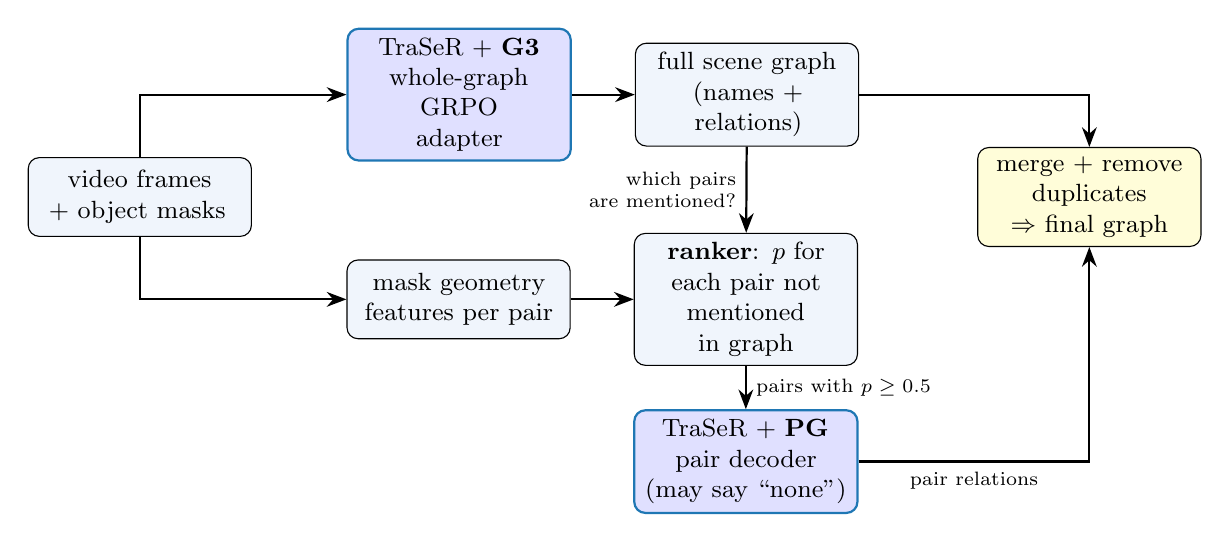
\begin{tikzpicture}[font=\small,node distance=0.55cm and 0.8cm,
  box/.style={draw,rounded corners,fill=soft,minimum height=1cm,align=center,text width=2.6cm},
  hl/.style={box,fill=blue!12,draw=ours,thick},
  ar/.style={-{Stealth[length=2.5mm]},thick}]
  \node[box] (in) {video frames\\+ object masks};
  \node[hl,right=1.2cm of in,yshift=1.3cm] (g3) {TraSeR + \textbf{G3}\\whole-graph GRPO\\adapter};
  \node[box,right=1.2cm of in,yshift=-1.3cm] (geo) {mask geometry\\features per pair};
  \node[box,right=of g3] (graph) {full scene graph\\(names + relations)};
  \node[box,right=of geo] (rank) {\textbf{ranker}: $p$ for\\each pair not\\mentioned in graph};
  \node[hl,below=of rank] (pg) {TraSeR + \textbf{PG}\\pair decoder\\(may say ``none'')};
  \node[box,right=1.5cm of graph,yshift=-1.3cm,fill=yellow!15] (merge) {merge + remove\\duplicates\\$\Rightarrow$ final graph};
  \draw[ar] (in) |- (g3);
  \draw[ar] (in) |- (geo);
  \draw[ar] (g3) -- (graph);
  \draw[ar] (geo) -- (rank);
  \draw[ar] (graph) -- node[left,font=\scriptsize,align=right] {which pairs\\are mentioned?} (rank);
  \draw[ar] (rank) -- node[right,font=\scriptsize] {pairs with $p\ge 0.5$} (pg);
  \draw[ar] (graph) -| (merge);
  \draw[ar] (pg) -| node[below,pos=0.25,font=\scriptsize] {pair relations} (merge);
\end{tikzpicture}
\caption{The current best pipeline (``G3 + PG''). Blue boxes are the two trained LoRA adapters on the same released TraSeR.}
\label{fig:pipeline}
\end{figure}

\hsec
\begin{table}[h]
\centering
\begin{tabular}{@{}llccc@{}}
\toprule
metric & benchmark & TraSeR (A0) & G3 & \textbf{G3 + PG} \\
\midrule
relation recall & SVG2test & 24.7 & 30.3\sig & \textbf{36.9}\sig \\
                & VidOR    & 9.2  & 9.8\sig  & \textbf{12.1}\sig \\
                & PVSG     & 9.7  & 10.5     & \textbf{14.1}\sig \\
\midrule
triplet recall  & SVG2test & 12.7 & 14.4\sig & \textbf{16.4}\sig \\
                & VidOR    & 6.4  & 7.2\sig  & \textbf{8.6}\sig \\
                & PVSG     & 4.7  & 5.5      & \textbf{6.4}\sig \\
\midrule
object accuracy & SVG2test & 49.9 & 49.9     & 49.9 \\
                & VidOR    & 77.3 & 79.1\sig & 79.1 \\
                & PVSG     & 58.3 & 57.3     & 57.3 \\
\midrule
relation F1     & SVG2test & 21.4 & 23.2     & 23.0 \\
                & VidOR    & 13.7 & 14.8\sig & \textbf{17.6}\sig \\
                & PVSG     & 7.3  & 7.7      & 8.3 \\
\bottomrule
\end{tabular}
\caption{Headline results (per-span tIoU $\ge 0.5$, duplicates merged, LLM-judged names and predicates). \sig{} = the 95\% paired
bootstrap CI of the difference from TraSeR excludes 0. Object names in G3 + PG come from the G3 graph, so its object accuracy equals
G3's. Precision change of G3 + PG vs.\ TraSeR: SVG2test $-2.1$ (CI $[-4.8,+0.6]$), VidOR $+5.6$\sig, PVSG $+0.1$.
F1 change: SVG2test $+1.7$ $[-0.9,+4.3]$, VidOR $+3.9$ $[3.2,4.7]$, PVSG $+1.0$ $[-0.5,+2.6]$.}
\label{tab:headline}
\end{table}

\begin{figure}[h]
\centering
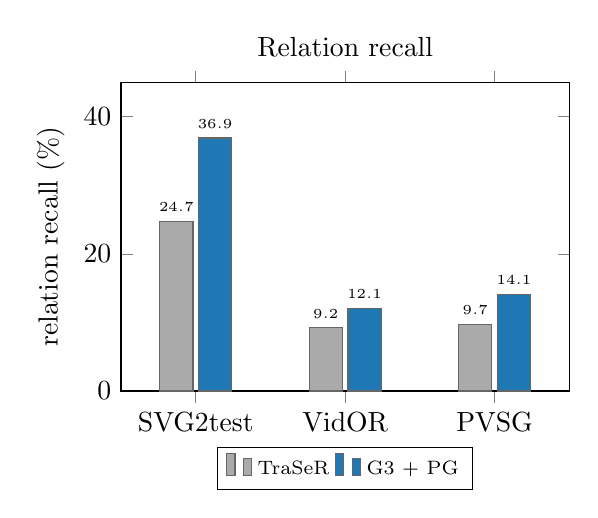
\begin{tikzpicture}
\begin{axis}[
  ybar, bar width=12pt, width=0.6\textwidth, height=5.5cm,
  symbolic x coords={SVG2test,VidOR,PVSG}, xtick=data,
  ymin=0, ymax=45, ylabel={relation recall (\%)},
  title={Relation recall},
  nodes near coords, nodes near coords style={font=\tiny},
  legend style={at={(0.5,-0.18)},anchor=north,legend columns=2,font=\scriptsize},
  enlarge x limits=0.25]
\addplot[fill=base,draw=black!60] coordinates {(SVG2test,24.7) (VidOR,9.2) (PVSG,9.7)};
\addplot[fill=ours,draw=black!60] coordinates {(SVG2test,36.9) (VidOR,12.1) (PVSG,14.1)};
\legend{TraSeR, G3 + PG}
\end{axis}
\end{tikzpicture}

\vspace{0.6em}
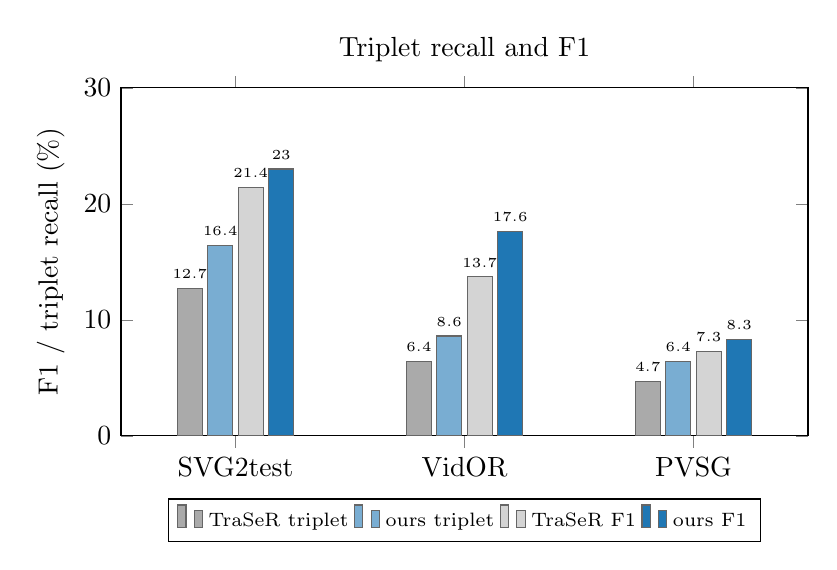
\begin{tikzpicture}
\begin{axis}[
  ybar, bar width=9pt, width=0.85\textwidth, height=6cm,
  symbolic x coords={SVG2test,VidOR,PVSG}, xtick=data,
  ymin=0, ymax=30, ylabel={F1 / triplet recall (\%)},
  title={Triplet recall and F1},
  nodes near coords, nodes near coords style={font=\tiny},
  legend style={at={(0.5,-0.18)},anchor=north,legend columns=4,font=\scriptsize},
  enlarge x limits=0.25]
\addplot[fill=base,draw=black!60] coordinates {(SVG2test,12.7) (VidOR,6.4) (PVSG,4.7)};
\addplot[fill=ours!60,draw=black!60] coordinates {(SVG2test,16.4) (VidOR,8.6) (PVSG,6.4)};
\addplot[fill=base!50,draw=black!60] coordinates {(SVG2test,21.4) (VidOR,13.7) (PVSG,7.3)};
\addplot[fill=ours,draw=black!60] coordinates {(SVG2test,23.0) (VidOR,17.6) (PVSG,8.3)};
\legend{TraSeR triplet, ours triplet, TraSeR F1, ours F1}
\end{axis}
\end{tikzpicture}
\caption{Headline comparison, TraSeR vs.\ G3 + PG. All recall gains are significant; the F1 gain is significant on VidOR only.}
\label{fig:headline}
\end{figure}

\section*{Robustness checks}
\begin{itemize}
  \item \textbf{Second seed.} Replacing PG by its seed-1 replicate (PGS1) gives the same headline: SVG2test F1 22.9 ($+1.6$
  n.s.), relation recall $+11.6$\sig, triplet recall $+3.6$\sig; VidOR F1 17.6\sig, relation recall $+2.9$\sig, triplet $+2.2$\sig;
  PVSG F1 8.4 ($+1.1$ n.s.), relation recall $+4.4$\sig, triplet $+1.8$\sig. (The seed-1 replicate of G3 itself was still running
  when this was written.)
  \item \textbf{Other tIoU definition.} Under union (merged-span) tIoU, relation recall still rises on all three: SVG2test
  25.2$\to$37.2, VidOR 5.7$\to$7.0, PVSG 6.3$\to$10.1.
  \item \textbf{Videos TraSeR never trained on.} On PVSG-clean (27 videos), relation recall rises 8.7$\to$12.6 ($+3.9$\sig); triplet
  recall 1.7$\to$2.7 and F1 7.0$\to$7.5 are not significant; object accuracy 50.4$\to$47.5 is not significant.
\end{itemize}

\lsec
\begin{keyidea}[What we can and cannot claim]
\textbf{Can claim:} one model, one configuration, trained only on TraSeR's data, finds significantly more true relations and more
fully correct triplets than TraSeR on all three benchmarks, with significantly higher precision and F1 on VidOR, and without
significantly hurting object naming anywhere. \textbf{Cannot (yet) claim:} a significant F1 gain on SVG2test or PVSG. With about 65
videos the confidence interval is roughly $\pm 2.6$ wide, so a gain of about 3 F1 points would be needed.
\end{keyidea}

\begin{summarybox}
G3 + PG combines whole-graph RL with ranked, abstaining, pair-level-RL pair decoding. Relation recall and triplet recall are
significantly higher than TraSeR on all three benchmarks; F1 is higher on all three, significantly on VidOR. The result holds with a
second pair-decoder seed, under the alternative tIoU definition (for recall), and on PVSG videos unseen by TraSeR (for recall).
\end{summarybox}

% ---------------------------------------------------------------------
\chapter{Error analysis: where are the remaining mistakes?}\label{ch:errors}

\qsec
After all this, what still goes wrong? Which errors are left, and are they the kind a better pair proposer could fix?

\tsec
We classified every true relation as \emph{found}, \emph{never mentioned} (no relation at all on that pair), \emph{wrong predicate},
\emph{other direction only}, \emph{wrong time}, or \emph{not in input} (an object beyond the 40-object cap), using exactly the
matching rules of the bootstrap. We also classified every \emph{prediction}: correct, or wrong because the pair has no true relation
at all, and so on.

\hsec
\begin{figure}[h]
\centering
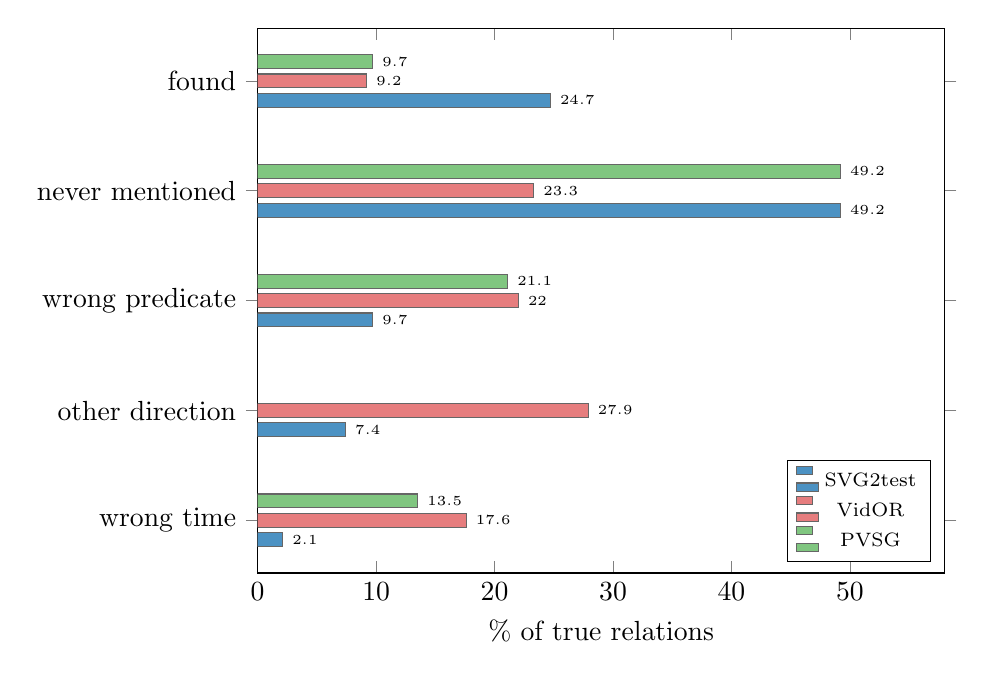
\begin{tikzpicture}
\begin{axis}[
  xbar, bar width=5pt, width=0.85\textwidth, height=8.5cm,
  symbolic y coords={wrong time,other direction,wrong predicate,never mentioned,found},
  ytick=data, xmin=0, xmax=58, xlabel={\% of true relations},
  nodes near coords, nodes near coords style={font=\tiny},
  legend style={at={(0.98,0.02)},anchor=south east,font=\scriptsize},
  enlarge y limits=0.12]
\addplot[fill=ours!80,draw=black!60] coordinates {(24.7,found) (49.2,never mentioned) (9.7,wrong predicate) (7.4,other direction) (2.1,wrong time)};
\addplot[fill=bad!60,draw=black!60] coordinates {(9.2,found) (23.3,never mentioned) (22.0,wrong predicate) (27.9,other direction) (17.6,wrong time)};
\addplot[fill=good!60,draw=black!60] coordinates {(9.7,found) (49.2,never mentioned) (21.1,wrong predicate) (13.5,wrong time)};
\legend{SVG2test, VidOR, PVSG}
\end{axis}
\end{tikzpicture}
\caption{Where TraSeR loses true relations. Categories not reported for a benchmark are omitted (for PVSG ``other direction'';
``not in input'' is 6.9\% on SVG2test and not shown).}
\label{fig:errors}
\end{figure}

\begin{figure}[h]
\centering
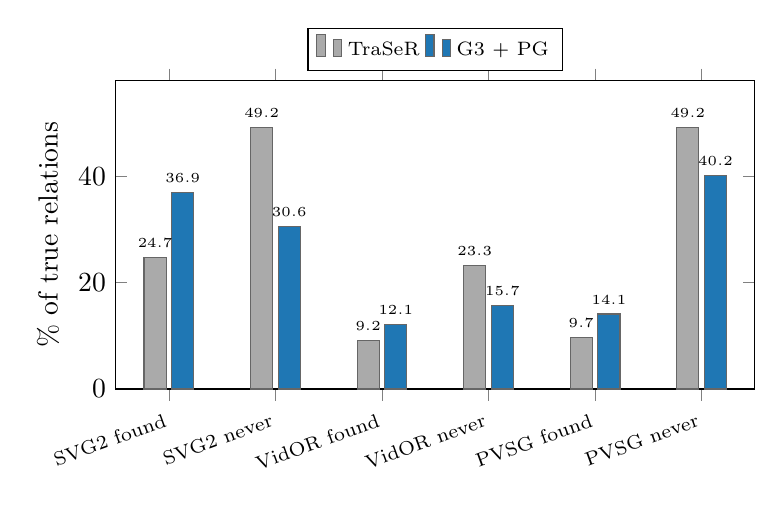
\begin{tikzpicture}
\begin{axis}[
  ybar, bar width=8pt, width=0.8\textwidth, height=5.5cm,
  symbolic x coords={SVG2 found,SVG2 never,VidOR found,VidOR never,PVSG found,PVSG never},
  xtick=data, x tick label style={font=\scriptsize,rotate=20,anchor=north east},
  ymin=0, ymax=58, ylabel={\% of true relations},
  nodes near coords, nodes near coords style={font=\tiny},
  legend style={at={(0.5,1.03)},anchor=south,legend columns=2,font=\scriptsize},
  enlarge x limits=0.1]
\addplot[fill=base,draw=black!60] coordinates {(SVG2 found,24.7) (SVG2 never,49.2) (VidOR found,9.2) (VidOR never,23.3) (PVSG found,9.7) (PVSG never,49.2)};
\addplot[fill=ours,draw=black!60] coordinates {(SVG2 found,36.9) (SVG2 never,30.6) (VidOR found,12.1) (VidOR never,15.7) (PVSG found,14.1) (PVSG never,40.2)};
\legend{TraSeR, G3 + PG}
\end{axis}
\end{tikzpicture}
\caption{``Found'' and ``never mentioned'' before and after our method. The pair stage converts never-mentioned pairs into hits.}
\label{fig:errors2}
\end{figure}

Two findings stand out.
\begin{itemize}
  \item \textbf{SVG2test and PVSG: most predictions sit on unlabelled pairs.} 65.9\% (SVG2test) and 66.1\% (PVSG) of TraSeR's
  \emph{own} predictions are on pairs that have no true relation at all. With G3 + PG this is 67.8\% on SVG2test (70.6\% for added
  pairs, 66.9\% for the base graph). Added pairs are correct 11.1\% of the time vs.\ 18.6\% for the base graph on SVG2test; on PVSG
  only 4.1\% of added predictions are correct. Pair \emph{selection} is the dominant precision error.
  \item \textbf{VidOR: convention and timing.} TraSeR's VidOR misses are led by ``other direction'' (27.9\%), and its predictions are
  often wrong in predicate (35.5\%) or time (17.1\%). But added pairs on VidOR are correct 55.2\% of the time -- better than the base
  graph's 30.8\%.
\end{itemize}

\section*{How much better could the ranker be?}
Within the training data (5-fold cross-validation by video), the ranker recovers 76.6\% of labelled PVD pairs at its own budget,
versus 86.8\% for a perfect ordering; on VidOR 87.0\% vs.\ 89.4\%. A diagnostic on test (used for no decision) shows a much larger gap
among \emph{unmentioned} pairs: SVG2test 39.4\% vs.\ 86.3\%, PVSG 40.7\% vs.\ 85.6\%. We also asked whether geometry could identify
TraSeR's \emph{own} false-positive pairs and prune them: on dev, F1 changed by at most $\pm 0.2$ for every threshold. Geometry
cannot tell which mentioned pairs are wrong.

\lsec
The biggest remaining lever on SVG2test and PVSG is choosing and describing pairs \emph{as the annotators would}; on VidOR it is the
labelling convention, the predicate vocabulary and the time spans. The next chapters show the ideas we tried for these, and what
is running now.

\begin{summarybox}
On SVG2test and PVSG two thirds of all predictions are on pairs annotators did not label, so pair selection limits precision. On
VidOR the remaining errors are direction convention, predicate vocabulary and timing. The ranker has headroom, but geometry alone
cannot spot wrong pairs that TraSeR already mentions.
\end{summarybox}

% =====================================================================
\part{Failures, open work, and the road ahead}
% =====================================================================

\chapter{What did not work, and why}\label{ch:failures}

\qsec
A research log full of successes is suspicious. Which ideas failed, and what did each failure teach us?

Figure~\ref{fig:tree} shows the whole project as a sequence of gates. Green ideas passed and became part of the method (or of the
evidence for it); red ideas failed a gate or were killed before using a GPU; orange ideas are still running.

\begin{figure}[p]
\centering
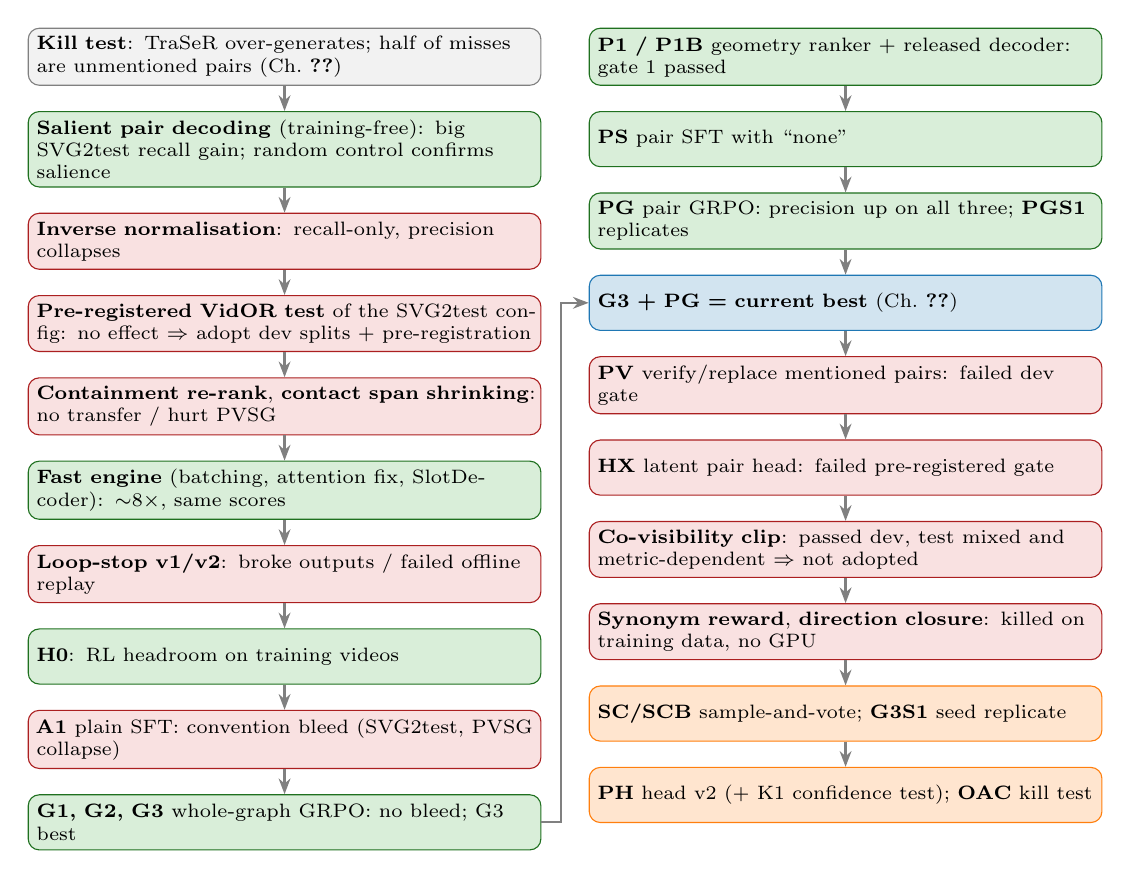
\begin{tikzpicture}[font=\scriptsize,node distance=0.32cm,
  st/.style={draw,rounded corners,align=left,text width=6.3cm,minimum height=0.7cm,inner sep=3pt},
  pass/.style={st,fill=good!18,draw=good!70!black},
  fail/.style={st,fill=bad!14,draw=bad!80!black},
  pen/.style={st,fill=pend!20,draw=pend},
  info/.style={st,fill=gray!10,draw=gray},
  ar/.style={-{Stealth[length=2mm]},thick,gray}]
  % left column: chronology part 1
  \node[info] (k) {\textbf{Kill test}: TraSeR over-generates; half of misses are unmentioned pairs (Ch.~\ref{ch:kill})};
  \node[pass,below=of k] (s) {\textbf{Salient pair decoding} (training-free): big SVG2test recall gain; random control confirms salience};
  \node[fail,below=of s] (inv) {\textbf{Inverse normalisation}: recall-only, precision collapses};
  \node[fail,below=of inv] (v) {\textbf{Pre-registered VidOR test} of the SVG2test config: no effect $\Rightarrow$ adopt dev splits + pre-registration};
  \node[fail,below=of v] (cont) {\textbf{Containment re-rank}, \textbf{contact span shrinking}: no transfer / hurt PVSG};
  \node[pass,below=of cont] (eng) {\textbf{Fast engine} (batching, attention fix, SlotDecoder): $\sim$8$\times$, same scores};
  \node[fail,below=of eng] (ls) {\textbf{Loop-stop v1/v2}: broke outputs / failed offline replay};
  \node[pass,below=of ls] (h0) {\textbf{H0}: RL headroom on training videos};
  \node[fail,below=of h0] (a1) {\textbf{A1} plain SFT: convention bleed (SVG2test, PVSG collapse)};
  \node[pass,below=of a1] (g) {\textbf{G1, G2, G3} whole-graph GRPO: no bleed; G3 best};
  % right column
  \node[pass,right=0.6cm of k] (p1) {\textbf{P1 / P1B} geometry ranker + released decoder: gate 1 passed};
  \node[pass,below=of p1] (ps) {\textbf{PS} pair SFT with ``none''};
  \node[pass,below=of ps] (pg) {\textbf{PG} pair GRPO: precision up on all three; \textbf{PGS1} replicates};
  \node[pass,below=of pg,fill=ours!20,draw=ours] (best) {\textbf{G3 + PG = current best} (Ch.~\ref{ch:best})};
  \node[fail,below=of best] (pv) {\textbf{PV} verify/replace mentioned pairs: failed dev gate};
  \node[fail,below=of pv] (hx) {\textbf{HX} latent pair head: failed pre-registered gate};
  \node[fail,below=of hx] (cv) {\textbf{Co-visibility clip}: passed dev, test mixed and metric-dependent $\Rightarrow$ not adopted};
  \node[fail,below=of cv] (syn) {\textbf{Synonym reward}, \textbf{direction closure}: killed on training data, no GPU};
  \node[pen,below=of syn] (sc) {\textbf{SC/SCB} sample-and-vote; \textbf{G3S1} seed replicate};
  \node[pen,below=of sc] (ph) {\textbf{PH} head v2 (+ K1 confidence test); \textbf{OAC} kill test};
  \foreach \a/\b in {k/s,s/inv,inv/v,v/cont,cont/eng,eng/ls,ls/h0,h0/a1,a1/g,p1/ps,ps/pg,pg/best,best/pv,pv/hx,hx/cv,cv/syn,syn/sc,sc/ph}
    \draw[ar] (\a) -- (\b);
  \draw[ar] (g.east) -- ++(0.25,0) |- (best.west);
\end{tikzpicture}
\caption{The project as a chain of gates, roughly in chronological order (left column first). Green: passed and kept. Red: failed or
killed. Orange: running when this book was written. Blue: the current best method.}
\label{fig:tree}
\end{figure}

\section{PV: letting the pair decoder check TraSeR's own pairs}
\tsec
The pair decoder never touched pairs TraSeR \emph{already} mentions. Since TraSeR over-generates on SVG2test and PVSG, perhaps PG
could verify them. Before seeing any number we wrote down three variants per mentioned pair -- BASE (keep TraSeR's relations),
VERIFY (drop them if PG says ``none''), REPLACE (use PG's relations instead) -- and a rule: choose the variant with the higher dev F1
only if it does not lower F1 on \emph{either} dev source; else keep BASE.

\hsec
On VidOR dev: BASE 7.1, VERIFY 5.7, REPLACE 34.9 (a huge jump). On PVD dev: BASE 22.2, VERIFY 18.4, REPLACE 17.6. VERIFY hurt both;
REPLACE is simply VidOR's convention leaking in through the video domain -- great on VidOR-style videos, harmful on PVD. The rule
said keep BASE, so the test decodes were \emph{never scored}.

\wsec
The pair decoder's hard negatives were unlabelled pairs the ranker liked, not ``pairs TraSeR mentioned wrongly''; mentioned pairs
were outside its training distribution. Also, PG's outputs carry VidOR's both-direction habit by domain: the share of both-direction
answers was 0.43 on SVG2test pairs and 0.81 on PVSG pairs, against true rates of 0.09 and 0.02.

\section{HX: a pair head reading the model's own hidden states}
\tsec
Instead of geometry only, read the language model's internal representation of each object (the average hidden state over its
block, from three layers) and train a small neural network to predict whether a pair is labelled -- alone (LAT) or combined with
geometry (LAT+GEO). Pre-registered rule: replace the geometry ranker only if recall at the same budget is higher on \emph{both} PVD
and VidOR in 5-fold cross-validation.

\hsec
PVD: GEO 76.4, LAT 75.9, LAT+GEO 76.9. VidOR: GEO 87.1, LAT 85.9, LAT+GEO 86.3. LAT+GEO won on PVD by 0.5 but lost on VidOR by 0.8.
\textbf{Gate failed}; the geometry ranker stayed, and no test list was changed.

\lsec
Averaged per-object states of the released model carry no extra ``will an annotator label this pair'' signal beyond geometry. A
better head should be trained on what the decoder gets \emph{right} (see head v2 in Chapter~\ref{ch:pending}), not on whether a label
exists.

\section{Co-visibility clipping of time spans}
\tsec
Clip every predicted span to the moments when both objects are actually visible; drop a relation if nothing is left.

\hsec
On dev it passed the rule (PVD F1 22.2$\to$23.2, CI $[+0.1,+2.0]$; VidOR 7.1$\to$7.2). While preparing PVSG we found and fixed a timing
bug in our own clipping script (masks were timed at the wrong frame rate, so only 65\% of true relations survived; after the fix
97.5\%). On test, G3 + PG + clip gave a dramatic VidOR jump (F1 25.6, $+11.9$\sig{} vs.\ TraSeR) and a small SVG2test gain, but lowered
PVSG recall ($-1.5$\sig). Under the union tIoU definition the VidOR gain vanished and PVSG dropped sharply (G3 + PG relation recall
10.1$\to$6.1).

\lsec
Clipping splits long spans at visibility gaps, which happens to match how VidOR's labels are cut into segments -- under per-span
tIoU only. It also cuts correct human-action spans at moments of occlusion. Because it hurts PVSG under both definitions and its
main gain depends on the metric definition, it was \textbf{not adopted} (we used test results only to exclude, never to include).

\section{Two ideas killed on training data before any GPU}
\paragraph{Synonym-aware reward.} Our reward requires exact predicate matches. Would counting synonyms help? On 80 dev videos we
looked at predictions on a labelled pair with temporal overlap but a different predicate. Most were genuinely different predicates
(VidOR: ``next to'' vs.\ ``in front of'' 21 times, ``above'' vs.\ ``on'' 15). Pure word-form variants (``holds''/``holding'') were only
1.3\% (PVD) and 1.4\% (VidOR) of all predictions. The ceiling was too low to justify retraining.

\paragraph{Direction closure.} Emit the inverse of symmetric predicates automatically? The training labels show that ``the other
direction'' is a labelling convention: the reverse pair is labelled 91.5\% of the time in VidOR but 13.1\% in PVD, and VidOR repeats
even non-symmetric predicates in both directions (``in front of'' 41\%). Any closure rule would help VidOR only by copying its
convention, at a precision cost on the sparse sources -- benchmark targeting under our rules.

\section{The earlier failures, collected}
\begin{itemize}
  \item The SVG2test-chosen training-free configuration did nothing on VidOR (Chapter~\ref{ch:salience}).
  \item Inverse normalisation and bidirectional completion: helpful only where labels are bidirectional (VidOR); on SVG2test the
  bidirectional transform lowered F1 from 20.1 to 14.6.
  \item Re-ranking by containment: designed on test analysis, did not transfer to PVSG.
  \item Contact-based span shrinking: hurt PVSG.
  \item The first two loop-stopping rules: broke outputs or failed replay (Chapter~\ref{ch:engine}).
  \item Plain SFT (A1): convention bleed (Chapter~\ref{ch:rl}).
  \item H2 (train on touching-only labels): the data contradicted its premise.
  \item G1: safe but under-trained -- a ``partial failure'' that motivated G3.
  \item Pruning TraSeR's own pairs by geometry: no effect on dev (Chapter~\ref{ch:errors}).
\end{itemize}

\begin{summarybox}
PV failed its dev gate; HX failed its pre-registered gate; co-visibility clipping passed dev but was excluded because it hurt PVSG
and its gain depended on the tIoU definition; synonym reward and direction closure were killed on training data. Several earlier
tricks only helped one benchmark. The common thread: ideas that copy one benchmark's convention fail the ``one configuration'' rule.
\end{summarybox}

% ---------------------------------------------------------------------
\chapter{Experiments in progress}\label{ch:pending}

The following experiments were designed, pre-registered and launched, but their results were not available when this book was
written. Each description includes the rule that will decide its fate, written down before any result was seen.

\begin{pendingbox}[G3S1 -- second seed of whole-graph GRPO]
The same G3 training with a different seed (training order, sampling, initialisation), using the final step-300 weights as for G3.
It tests whether the G3 part of the headline is robust to training randomness, as PGS1 showed for PG.
\end{pendingbox}

\begin{pendingbox}[SC -- sample-and-vote decoding]
\textbf{Idea.} G3 was trained on \emph{sampled} graphs (temperature 1.0), but we score its \emph{greedy} graph. Relations the model
produces consistently across many samples may be more reliable than one greedy pass.

\textbf{Design.} For each video: the greedy graph plus 8 samples with the training settings. Aggregators fixed in advance:
\begin{itemize}
  \item \textbf{VOTE($m$)}, $m\in\{3,5,7\}$: keep a (subject, predicate, object) if at least $m$ of the 9 graphs contain it; its spans
  come from the instance that agrees best in time with the others.
  \item \textbf{MBR} (minimum Bayes risk): pick the single graph that has the highest average F1 against the other 8.
\end{itemize}
\textbf{Gate.} On the 80 dev videos, mean F1 change $\ge 0$ on both sources \emph{and} the pooled 95\% CI above 0; the best passing
aggregator wins; if none pass, the test samples are not scored. \textbf{Control (SCB):} the same procedure on the released TraSeR, to
separate ``voting helps any model'' from ``voting helps the RL model''. A diagnostic is computed first: if relations on unlabelled
pairs are as consistent across samples as correct ones, voting cannot fix SVG2test/PVSG precision.
\end{pendingbox}

\begin{pendingbox}[PH -- head v2, a reward-trained pair head]
\textbf{Idea.} HX failed because it predicted ``is this pair labelled''. What matters is whether \emph{adding} a pair's decoded
relations helps. Head v2 learns, on training videos, the fraction of a pair's decoded relations that are correct, from geometry,
ranker score, rank, and features of the decode itself (number of relations, distinct predicates, both-directions flag, span length,
the predicate's historical precision, and two decoder-confidence features).

\textbf{Selection rule (no tuning).} Add a pair's relations if and only if the predicted precision exceeds $F1_{\text{dev}}/2$ -- the
rule derived in Chapter~\ref{ch:measure}: adding a relation that is correct with probability $q$ raises F1 exactly when $q > F1/2$.

\textbf{Gate.} On dev, versus the current $p\ge 0.5$ rule: mean F1 change $\ge 0$ on both sources and pooled CI above 0. Only then is
the head applied, once, to the existing test decodes.

\textbf{Kill test K1, ``does the decoder know its own hits?''} If combining geometry with the decoder's probability of answering
``none'' does not beat geometry alone on both sources, and if relation log-probabilities separate correct from unlabelled-pair
relations with AUROC below 0.60, ideas based on decoder confidence are killed.
\end{pendingbox}

\begin{pendingbox}[OAC -- object-ablation credit (kill test)]
\textbf{Idea.} Because each object has its own block, we can ask: if we replace object $s$'s block by an ``average object'', how much
does the model's confidence in a relation about $s$ drop? A relation that does not depend on its own objects is probably not
grounded in the video. This could become a label-free reward on pairs annotators did not label.

\textbf{Measure.} For each relation, $\delta = \min(\text{lp}-\text{lp}_s,\ \text{lp}-\text{lp}_o)$, the drop in average log-probability
per token of its predicate and span tokens when the subject or object block is replaced.

\textbf{Positive control.} Median $\delta$ on correct relations must exceed 0.1 nats per token, else the test is uninformative.
\textbf{Kill OAC} if any of: (a) $\delta$ separates correct from unlabelled-pair relations with AUROC below 0.60, or no better than the
geometry ranker; (b) $\delta$ differs more between data sources than between correct and wrong relations; (c) a dev filter
``drop if $\delta < d$'' (with $d$ chosen on one half of dev, checked on the other) does not raise F1 on both sources.
\end{pendingbox}

% ---------------------------------------------------------------------
\chapter{Future directions}\label{ch:future}

Two literature scouts surveyed recent work and proposed next steps. Their main suggestions are summarised here; all respect the
project's rules (same data, one configuration, dev-gated).

\section{Reinforcement-learning ideas}
\begin{enumerate}
  \item \textbf{Object-ablation credit (OAC)} -- the top pick, now being kill-tested (Chapter~\ref{ch:pending}). It targets the
  dominant SVG2test/PVSG error (predictions on unlabelled pairs) with a signal that does not depend on label density. It uses an
  intervention that only an object-block model like TraSeR allows. Main risk: predictions on unlabelled pairs may be well grounded
  but simply not annotated; then no label-free reward can fix measured precision.
  \item \textbf{Relation-level calibrated confidence}: the model attaches a confidence to each relation and is rewarded with a proper
  scoring rule; one global threshold is set on dev.
  \item \textbf{Relation-keyed advantages}: in whole-graph GRPO, give each relation line its own advantage by comparing it with the
  same pair in the other samples, instead of one advantage for the whole graph.
  \item \textbf{Span-sensitive temporal reward}: add a term that still gives a learning signal when a predicted span does not overlap
  the truth at all (tIoU 0), aimed at VidOR and PVSG timing errors.
  \item \textbf{Consensus pseudo-reward}: reward relations that recur across samples on unlabelled training pairs (risky: it can
  reinforce the model's own biases).
\end{enumerate}

\section{Architecture ideas}
The architecture scout's top proposal is to move the pipeline \emph{inside} the language model (Figure~\ref{fig:future}):
\textbf{pair-branch decoding} with a \textbf{reward-trained proposer}.
\begin{itemize}
  \item After the object blocks (and optionally the model's own whole graph), add special \texttt{<pair>} tokens for candidate pairs.
  Each \texttt{<pair>} token can see both full object blocks and the graph so far.
  \item A tiny network (about 2 million parameters) reads the \texttt{<pair>} token's internal state and scores the pair. It is
  trained on the \emph{pair decoder's reward} -- does decoding this pair help? -- not on ``is this pair labelled'' (the lesson of HX).
  \item The top pairs are decoded as parallel \emph{branches} that share the same prefix but cannot see each other, using the PG
  adapter with its ``none'' option.
\end{itemize}
Proposed kill tests first: (A) does combining geometry with the decoder's own ``none'' probability beat geometry alone on both
sources? (B) do \texttt{<pair>}-token states carry pair information beyond geometry? If (A) fails, only an efficiency story remains.

\begin{figure}[h]
\centering
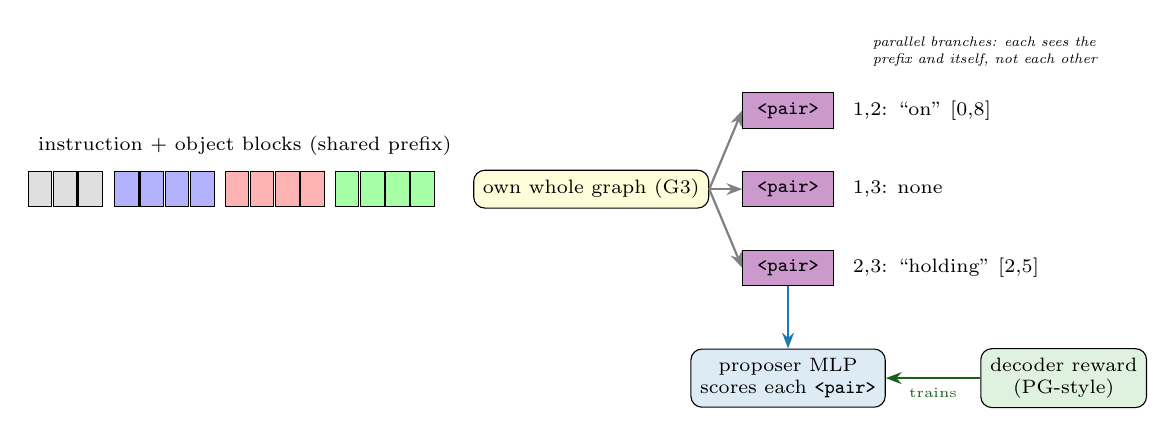
\begin{tikzpicture}[font=\scriptsize,
  tok/.style={draw,minimum width=0.3cm,minimum height=0.45cm,inner sep=0},
  ar/.style={-{Stealth[length=2mm]},thick}]
  \foreach \i in {0,...,2} \node[tok,fill=gray!25] at (\i*0.32,0) {};
  \foreach \i in {0,...,3} \node[tok,fill=blue!30] at (1.1+\i*0.32,0) {};
  \foreach \i in {0,...,3} \node[tok,fill=red!30] at (2.5+\i*0.32,0) {};
  \foreach \i in {0,...,3} \node[tok,fill=green!35] at (3.9+\i*0.32,0) {};
  \node[draw,rounded corners,fill=yellow!15,minimum height=0.45cm] (gr) at (7.0,0) {own whole graph (G3)};
  \node[above,font=\scriptsize] at (2.6,0.3) {instruction + object blocks (shared prefix)};
  % pair tokens
  \node[tok,fill=violet!40,minimum width=1.15cm] (p1) at (9.5,1.0) {\texttt{<pair>}};
  \node[tok,fill=violet!40,minimum width=1.15cm] (p2) at (9.5,0) {\texttt{<pair>}};
  \node[tok,fill=violet!40,minimum width=1.15cm] (p3) at (9.5,-1.0) {\texttt{<pair>}};
  \draw[ar,gray] (gr.east) -- (p1.west); \draw[ar,gray] (gr.east) -- (p2.west); \draw[ar,gray] (gr.east) -- (p3.west);
  \node[anchor=west] at (10.2,1.0) {1,2: ``on'' [0,8]};
  \node[anchor=west] at (10.2,0) {1,3: none};
  \node[anchor=west] at (10.2,-1.0) {2,3: ``holding'' [2,5]};
  % proposer
  \node[draw,rounded corners,fill=ours!15,align=center] (prop) at (9.5,-2.4) {proposer MLP\\scores each \texttt{<pair>}};
  \draw[ar,ours] (p3.south) -- (prop.north);
  \node[draw,rounded corners,fill=good!15,align=center] (rw) at (13.0,-2.4) {decoder reward\\(PG-style)};
  \draw[ar,good!60!black] (rw.west) -- node[below,font=\tiny] {trains} (prop.east);
  \node[align=left,font=\tiny\itshape] at (12.0,1.75) {parallel branches: each sees the\\prefix and itself, not each other};
\end{tikzpicture}
\caption{Planned future architecture: pair-branch decoding inside one model pass. The proposer reads the model's own pair tokens
and is trained on the pair decoder's reward.}
\label{fig:future}
\end{figure}

Other architecture ideas, each with its own cheap kill test: per-time-window pair tokens carrying directed geometry (aimed at VidOR
predicate and timing errors); a set-structured object prefix so object order does not matter (a probe found little order effect);
per-object naming branches (object accuracy on SVG2test is flat at 49.9); and an adaptive budget of visual tokens to fit long PVSG
videos.

\begin{summarybox}
Next steps aim at the error that remains: predictions on pairs annotators did not label. The leading RL idea (OAC) asks whether a
relation really depends on its objects. The leading architecture idea moves the ranker and pair decoder inside the language model,
with a proposer trained on what the decoder gets right.
\end{summarybox}

% ---------------------------------------------------------------------
\chapter{Lessons}\label{ch:lessons}

\begin{enumerate}
  \item \textbf{Measure before you cure.} The kill test showed the problem was \emph{which pairs}, not \emph{how many relations}.
  \item \textbf{Every benchmark is a convention.} SVG2test, VidOR and PVSG disagree on direction, density, vocabulary and timing. A
  gain that comes from copying one convention is not a better model.
  \item \textbf{Write the rule before you see the result.} The pre-registered VidOR test killed a method that looked excellent on the
  benchmark where it was designed. Pre-registration also killed PV and HX cleanly.
  \item \textbf{Use fair controls.} Random pairs (for salience) and plain SFT (for RL) told us which part of each gain was real.
  \item \textbf{RL can improve without copying.} On the same data, SFT imported VidOR's style everywhere; RL with a KL penalty did not.
  \item \textbf{Factor hard problems.} Separating ``which pairs'' from ``what to say about a pair'' gave each part a clean learning
  signal and produced the gains that hold on all three benchmarks.
  \item \textbf{Engineering is part of the science.} An 8$\times$ faster engine, verified to give the same scores, made the RL
  experiments possible.
  \item \textbf{Report what you cannot claim.} Our F1 gains on SVG2test and PVSG are positive but not significant; that is stated as
  plainly as the significant gains.
\end{enumerate}

\begin{bestbox}
\textbf{G3 + PG.} TraSeR with a whole-graph GRPO adapter (G3) writes the scene graph; a geometry ranker trained on TraSeR's own
training labels proposes unmentioned pairs with $p \ge 0.5$; a pair-level GRPO adapter (PG), warm-started from a pair SFT adapter
that can answer ``none'', describes them; the outputs are merged and deduplicated. One configuration for all three benchmarks.
Relation recall: SVG2test 24.7$\to$36.9\sig, VidOR 9.2$\to$12.1\sig, PVSG 9.7$\to$14.1\sig. Triplet recall: 12.7$\to$16.4\sig,
6.4$\to$8.6\sig, 4.7$\to$6.4\sig. F1: 21.4$\to$23.0 (n.s.), 13.7$\to$17.6\sig, 7.3$\to$8.3 (n.s.). Object accuracy: 49.9$\to$49.9,
77.3$\to$79.1\sig, 58.3$\to$57.3 (n.s.).
\end{bestbox}

% =====================================================================
\appendix
\chapter{Experiment code names}\label{app:codes}
\begin{center}
\small
\begin{tabular}{@{}>{\bfseries}l p{12.5cm}@{}}
\toprule
code & what it is \\
\midrule
A0 & Baseline: released TraSeR run through our fast engine on all three benchmarks (with a separate PVSG re-run, A0P, after a memory fix). \\
A1 & Plain SFT control on 300 VidOR + 300 PVD training samples; caused convention bleed. \\
A2 & Designed: SFT with a per-source style tag. No result for it appears in the log; a per-benchmark tag would also conflict with the one-configuration rule. \\
H0 & Pre-check of RL headroom: greedy vs.\ 8 samples on training videos, scored by the reward. Passed. \\
G1 & Whole-graph GRPO, 150 steps, lr $10^{-5}$, 50/50 VidOR/PVD. Safe but under-trained. \\
G2 & As G1 with TraSeR's natural source mix. Same small, convention-independent gain. \\
G3 & Whole-graph GRPO, lr $3\times10^{-5}$, 300 steps. Best whole-graph model; part of the headline. \\
G3S1 & G3 with training seed 1. Running. \\
P1 & Released TraSeR decodes pairs proposed by a geometry ranker (trained on 289 PVD videos), top-$K$ comparison with contact and random. Gate 1 passed. \\
P1B & As P1 with the ranker trained on all relation-labelled training data and the $p\ge0.5$ rule. \\
PS & Pair-decoder LoRA trained by SFT, with ``none'' targets on hard negatives. \\
PG & Pair-level GRPO warm-started from PS; abstention rewarded on hard negatives. Part of the headline. \\
PGS1 & PG with training seed 1. Replicated PG's precision gain over PS. \\
PV & PG applied to pairs TraSeR already mentions (verify / replace). Failed its pre-registered dev gate. \\
HX & Pair head on the model's hidden states (LAT, LAT+GEO). Failed its pre-registered gate. \\
SC & Sample-and-vote decoding on G3 (VOTE / MBR aggregators). Running. \\
SCB & The same on the released TraSeR, as a control. Running. \\
PH & Data for head v2, a pair head trained on the decoder's reward. Running. \\
K1 & Kill test: does the decoder's own confidence identify its correct pairs? Inside PH. \\
OAC & Kill test for object-ablation credit, inside the SCB run. Running. \\
GEO & The geometry ranker (gradient-boosted trees on mask-geometry features). \\
LAT & Latent (hidden-state) pair head tested in HX. \\
\bottomrule
\end{tabular}
\end{center}
Earlier, unnamed runs (Chapters~\ref{ch:kill}--\ref{ch:engine}) include the original kill test, pair decoding with both prompts,
the random-pair control, the benchmark runs on PVSG and VidOR, and a series of engine speed tests and profiles.

\chapter{Glossary}\label{app:glossary}
\begin{description}[style=nextline,leftmargin=0.6cm,font=\bfseries]
\item[Abstention (``none'')] The pair decoder answering that a pair has no relation worth stating.
\item[Adapter] The small trained correction added to a frozen model by LoRA; can be switched on and off.
\item[Advantage] In GRPO, an answer's reward minus the average reward of its group.
\item[Annotation convention] The habits of a dataset's labellers: how many relations per pair, whether both directions are written,
which words are used, how spans are cut.
\item[Benchmark] A fixed test set with labels, used to compare methods.
\item[Benchmark targeting] Giving a system special settings or knowledge for a particular test. Forbidden here.
\item[Bootstrap (paired)] Resampling test videos with replacement many times to estimate a confidence interval for a difference
between two systems scored on the same videos.
\item[Confidence interval (CI)] A range that likely contains the true value; here the 95\% range from 2000 bootstrap resamples.
\item[Contact filter] Dropping predicted relations between objects whose masks never touch.
\item[Convention bleed] A model trained on mixed-convention data applying one dataset's convention everywhere.
\item[Dev split] Training videos held out from training and used to make decisions (40 PVD + 40 VidOR).
\item[Duplicate merging (dedup)] Merging identical (subject, predicate, object) relations before scoring.
\item[F1] Harmonic mean of precision and recall: $2PR/(P+R)$.
\item[Fine-tuning] Continuing to train an already trained model on new examples.
\item[GRPO] Group Relative Policy Optimisation: RL that samples a group of answers per input and uses reward minus the group mean as
the learning signal.
\item[Greedy decoding] Always choosing the most probable next token.
\item[Hard negative] An unlabelled pair that the ranker nevertheless finds plausible; used to teach abstention.
\item[KL penalty] A term that keeps the trained model's token probabilities close to the original model's.
\item[Kill test] A cheap experiment designed to reject a hypothesis quickly if it is wrong.
\item[KV cache] The stored internal ``memory'' of what a language model has already read, reused at every generation step.
\item[LLM judge] A separate language model that decides whether two labels (for example two predicates) mean the same thing.
\item[LoRA] Low-Rank Adaptation: training a small product of thin matrices instead of all the model's weights.
\item[Mask] A pixel outline of an object in each frame.
\item[Object block] TraSeR's group of visual tokens describing one object's trajectory.
\item[Pair query] Feeding TraSeR only two object blocks and asking it to describe their relations.
\item[Per-span / union tIoU] Two ways to score timing when a relation has several spans: best single span match, or one IoU after
merging spans.
\item[Precision] Fraction of predictions that are correct.
\item[Pre-registration] Writing down a decision rule before seeing the results it will be applied to.
\item[Predicate] The relation word, such as ``on'', ``holding'', ``riding''.
\item[Ranker] The model that scores how likely a pair of objects is to have a labelled relation (here, from mask geometry).
\item[Recall] Fraction of true relations that are found.
\item[Reward] The score given to a model's answer in reinforcement learning.
\item[Reward hacking] A model finding a degenerate output that scores well without being good.
\item[Salience] How likely humans are to mention something; here, which object pairs annotators describe.
\item[Sampling, temperature] Choosing the next token at random according to the model's probabilities; temperature controls how
spread out the choice is.
\item[Scene graph] Objects plus relations between them; in video, relations have time spans.
\item[Seed] The starting value of a random number generator; changing it changes all random choices in training.
\item[SFT] Supervised fine-tuning: training the model to reproduce target answers.
\item[Smoke test] A quick local test that a change works before spending GPU time.
\item[Temporal IoU (tIoU)] Overlap of two time spans divided by the time they cover together.
\item[Token] A small chunk of text (or a visual patch) that a language model reads or writes.
\item[Triplet] (subject name, predicate, object name); triplet recall requires the relation and both names to be correct.
\item[Vision-language model (VLM)] A language model that can also read images or video through visual tokens.
\end{description}

\end{document}
